\begin{figure}[H] \centering % Created by tikzDevice version 0.12.4 on 2023-08-13 18:11:24
% !TEX encoding = UTF-8 Unicode
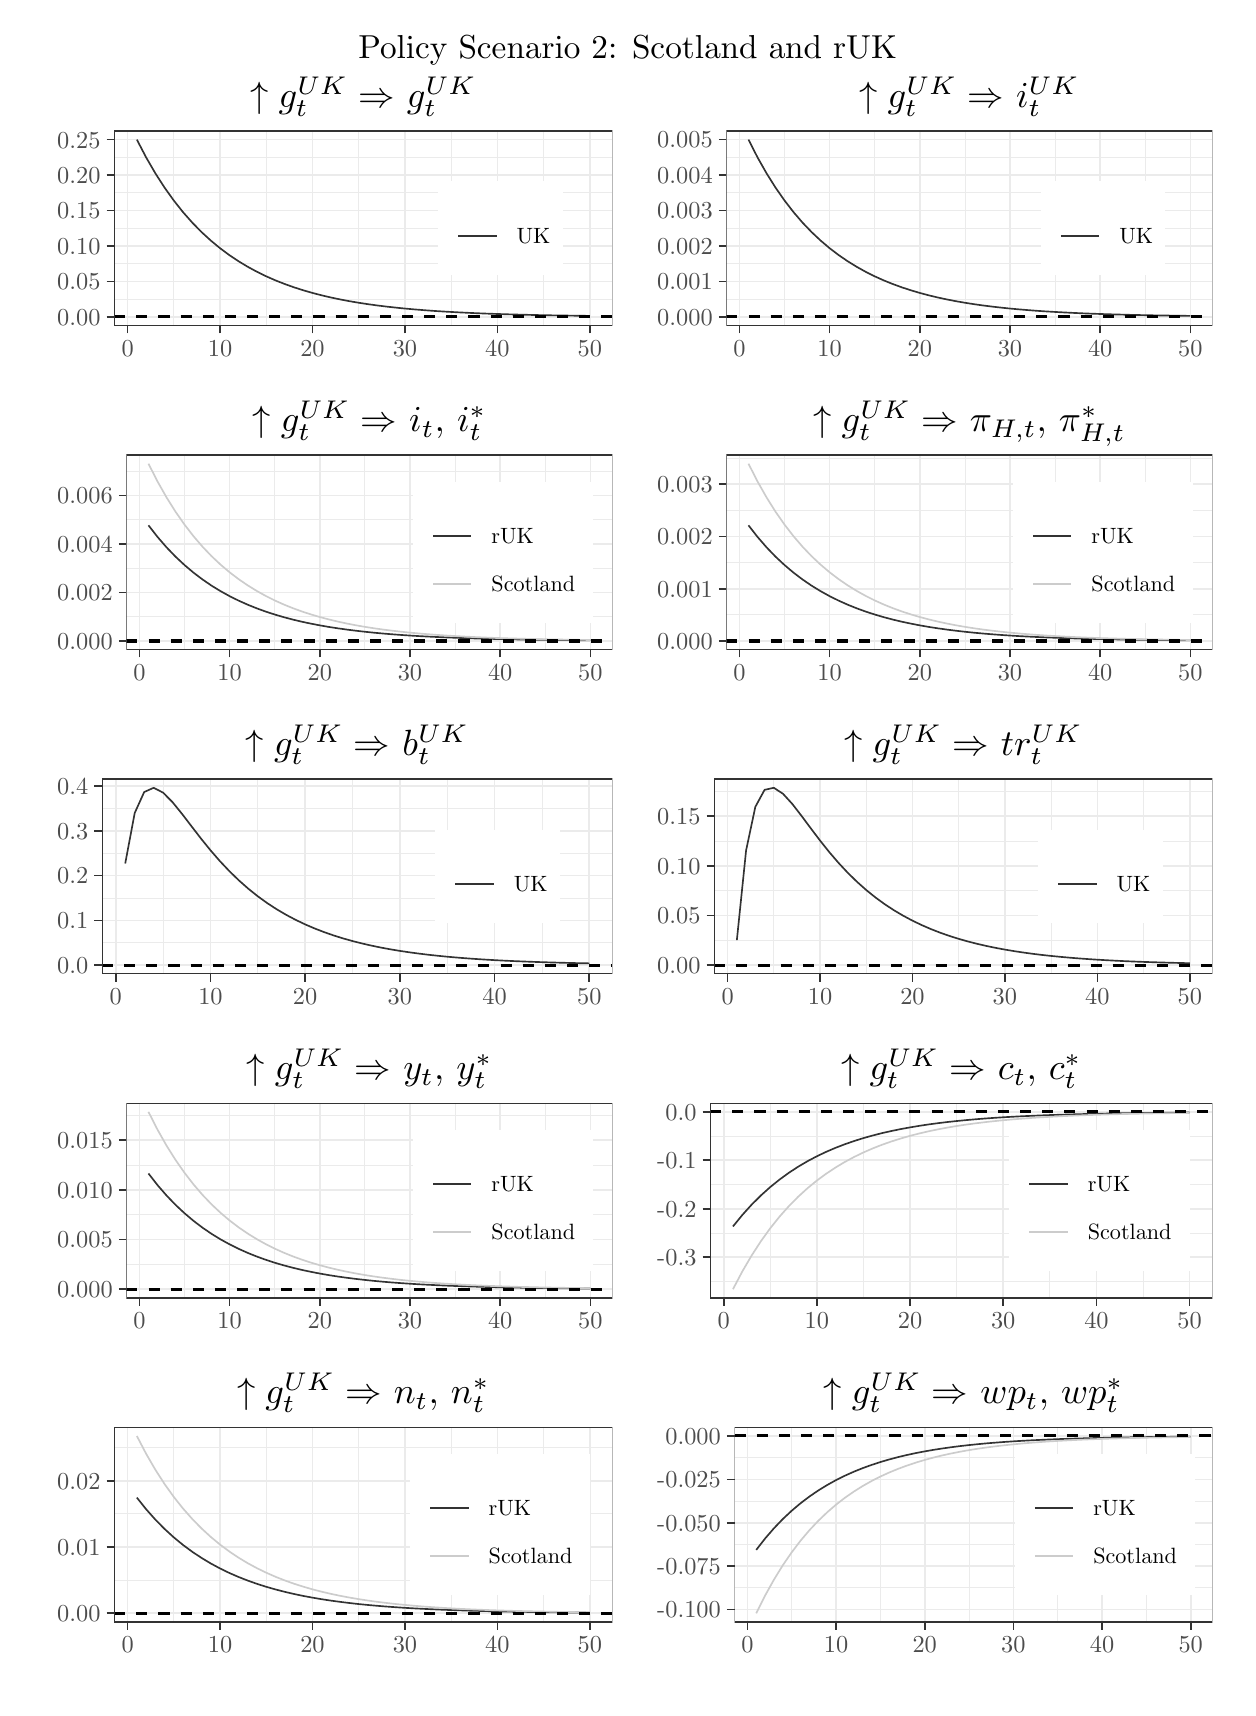
\begin{tikzpicture}[x=1pt,y=1pt]
\definecolor{fillColor}{RGB}{255,255,255}
\path[use as bounding box,fill=fillColor,fill opacity=0.00] (0,0) rectangle (433.62,599.84);
\begin{scope}
\path[clip] (  0.00,468.44) rectangle (216.81,585.55);
\definecolor{drawColor}{RGB}{255,255,255}
\definecolor{fillColor}{RGB}{255,255,255}

\path[draw=drawColor,line width= 0.6pt,line join=round,line cap=round,fill=fillColor] (  0.00,468.44) rectangle (216.81,585.55);
\end{scope}
\begin{scope}
\path[clip] ( 31.27,492.12) rectangle (211.31,562.59);
\definecolor{fillColor}{RGB}{255,255,255}

\path[fill=fillColor] ( 31.27,492.12) rectangle (211.31,562.59);
\definecolor{drawColor}{gray}{0.92}

\path[draw=drawColor,line width= 0.3pt,line join=round] ( 31.27,501.73) --
	(211.31,501.73);

\path[draw=drawColor,line width= 0.3pt,line join=round] ( 31.27,514.54) --
	(211.31,514.54);

\path[draw=drawColor,line width= 0.3pt,line join=round] ( 31.27,527.36) --
	(211.31,527.36);

\path[draw=drawColor,line width= 0.3pt,line join=round] ( 31.27,540.17) --
	(211.31,540.17);

\path[draw=drawColor,line width= 0.3pt,line join=round] ( 31.27,552.98) --
	(211.31,552.98);

\path[draw=drawColor,line width= 0.3pt,line join=round] ( 52.81,492.12) --
	( 52.81,562.59);

\path[draw=drawColor,line width= 0.3pt,line join=round] ( 86.22,492.12) --
	( 86.22,562.59);

\path[draw=drawColor,line width= 0.3pt,line join=round] (119.62,492.12) --
	(119.62,562.59);

\path[draw=drawColor,line width= 0.3pt,line join=round] (153.02,492.12) --
	(153.02,562.59);

\path[draw=drawColor,line width= 0.3pt,line join=round] (186.43,492.12) --
	(186.43,562.59);

\path[draw=drawColor,line width= 0.6pt,line join=round] ( 31.27,495.32) --
	(211.31,495.32);

\path[draw=drawColor,line width= 0.6pt,line join=round] ( 31.27,508.14) --
	(211.31,508.14);

\path[draw=drawColor,line width= 0.6pt,line join=round] ( 31.27,520.95) --
	(211.31,520.95);

\path[draw=drawColor,line width= 0.6pt,line join=round] ( 31.27,533.76) --
	(211.31,533.76);

\path[draw=drawColor,line width= 0.6pt,line join=round] ( 31.27,546.58) --
	(211.31,546.58);

\path[draw=drawColor,line width= 0.6pt,line join=round] ( 31.27,559.39) --
	(211.31,559.39);

\path[draw=drawColor,line width= 0.6pt,line join=round] ( 36.11,492.12) --
	( 36.11,562.59);

\path[draw=drawColor,line width= 0.6pt,line join=round] ( 69.52,492.12) --
	( 69.52,562.59);

\path[draw=drawColor,line width= 0.6pt,line join=round] (102.92,492.12) --
	(102.92,562.59);

\path[draw=drawColor,line width= 0.6pt,line join=round] (136.32,492.12) --
	(136.32,562.59);

\path[draw=drawColor,line width= 0.6pt,line join=round] (169.72,492.12) --
	(169.72,562.59);

\path[draw=drawColor,line width= 0.6pt,line join=round] (203.13,492.12) --
	(203.13,562.59);
\definecolor{drawColor}{gray}{0.20}

\path[draw=drawColor,line width= 0.6pt,line join=round] ( 39.45,559.39) --
	( 42.79,552.98) --
	( 46.13,547.22) --
	( 49.47,542.03) --
	( 52.81,537.36) --
	( 56.15,533.15) --
	( 59.50,529.37) --
	( 62.84,525.96) --
	( 66.18,522.90) --
	( 69.52,520.14) --
	( 72.86,517.66) --
	( 76.20,515.43) --
	( 79.54,513.42) --
	( 82.88,511.61) --
	( 86.22,509.98) --
	( 89.56,508.51) --
	( 92.90,507.20) --
	( 96.24,506.01) --
	( 99.58,504.94) --
	(102.92,503.98) --
	(106.26,503.11) --
	(109.60,502.33) --
	(112.94,501.63) --
	(116.28,501.00) --
	(119.62,500.43) --
	(122.96,499.92) --
	(126.30,499.46) --
	(129.64,499.05) --
	(132.98,498.68) --
	(136.32,498.34) --
	(139.66,498.04) --
	(143.00,497.77) --
	(146.34,497.52) --
	(149.68,497.30) --
	(153.02,497.11) --
	(156.36,496.93) --
	(159.70,496.77) --
	(163.04,496.62) --
	(166.38,496.49) --
	(169.72,496.38) --
	(173.06,496.27) --
	(176.40,496.18) --
	(179.74,496.09) --
	(183.08,496.01) --
	(186.43,495.94) --
	(189.77,495.88) --
	(193.11,495.83) --
	(196.45,495.78) --
	(199.79,495.73) --
	(203.13,495.69);
\definecolor{drawColor}{RGB}{0,0,0}

\path[draw=drawColor,line width= 1.1pt,dash pattern=on 4pt off 4pt ,line join=round] ( 31.27,495.32) -- (211.31,495.32);
\definecolor{drawColor}{gray}{0.20}

\path[draw=drawColor,line width= 0.6pt,line join=round,line cap=round] ( 31.27,492.12) rectangle (211.31,562.59);
\end{scope}
\begin{scope}
\path[clip] (  0.00,  0.00) rectangle (433.62,599.84);
\definecolor{drawColor}{gray}{0.30}

\node[text=drawColor,anchor=base east,inner sep=0pt, outer sep=0pt, scale=  0.88] at ( 26.32,492.29) {0.00};

\node[text=drawColor,anchor=base east,inner sep=0pt, outer sep=0pt, scale=  0.88] at ( 26.32,505.11) {0.05};

\node[text=drawColor,anchor=base east,inner sep=0pt, outer sep=0pt, scale=  0.88] at ( 26.32,517.92) {0.10};

\node[text=drawColor,anchor=base east,inner sep=0pt, outer sep=0pt, scale=  0.88] at ( 26.32,530.73) {0.15};

\node[text=drawColor,anchor=base east,inner sep=0pt, outer sep=0pt, scale=  0.88] at ( 26.32,543.55) {0.20};

\node[text=drawColor,anchor=base east,inner sep=0pt, outer sep=0pt, scale=  0.88] at ( 26.32,556.36) {0.25};
\end{scope}
\begin{scope}
\path[clip] (  0.00,  0.00) rectangle (433.62,599.84);
\definecolor{drawColor}{gray}{0.20}

\path[draw=drawColor,line width= 0.6pt,line join=round] ( 28.52,495.32) --
	( 31.27,495.32);

\path[draw=drawColor,line width= 0.6pt,line join=round] ( 28.52,508.14) --
	( 31.27,508.14);

\path[draw=drawColor,line width= 0.6pt,line join=round] ( 28.52,520.95) --
	( 31.27,520.95);

\path[draw=drawColor,line width= 0.6pt,line join=round] ( 28.52,533.76) --
	( 31.27,533.76);

\path[draw=drawColor,line width= 0.6pt,line join=round] ( 28.52,546.58) --
	( 31.27,546.58);

\path[draw=drawColor,line width= 0.6pt,line join=round] ( 28.52,559.39) --
	( 31.27,559.39);
\end{scope}
\begin{scope}
\path[clip] (  0.00,  0.00) rectangle (433.62,599.84);
\definecolor{drawColor}{gray}{0.20}

\path[draw=drawColor,line width= 0.6pt,line join=round] ( 36.11,489.37) --
	( 36.11,492.12);

\path[draw=drawColor,line width= 0.6pt,line join=round] ( 69.52,489.37) --
	( 69.52,492.12);

\path[draw=drawColor,line width= 0.6pt,line join=round] (102.92,489.37) --
	(102.92,492.12);

\path[draw=drawColor,line width= 0.6pt,line join=round] (136.32,489.37) --
	(136.32,492.12);

\path[draw=drawColor,line width= 0.6pt,line join=round] (169.72,489.37) --
	(169.72,492.12);

\path[draw=drawColor,line width= 0.6pt,line join=round] (203.13,489.37) --
	(203.13,492.12);
\end{scope}
\begin{scope}
\path[clip] (  0.00,  0.00) rectangle (433.62,599.84);
\definecolor{drawColor}{gray}{0.30}

\node[text=drawColor,anchor=base,inner sep=0pt, outer sep=0pt, scale=  0.88] at ( 36.11,481.11) {0};

\node[text=drawColor,anchor=base,inner sep=0pt, outer sep=0pt, scale=  0.88] at ( 69.52,481.11) {10};

\node[text=drawColor,anchor=base,inner sep=0pt, outer sep=0pt, scale=  0.88] at (102.92,481.11) {20};

\node[text=drawColor,anchor=base,inner sep=0pt, outer sep=0pt, scale=  0.88] at (136.32,481.11) {30};

\node[text=drawColor,anchor=base,inner sep=0pt, outer sep=0pt, scale=  0.88] at (169.72,481.11) {40};

\node[text=drawColor,anchor=base,inner sep=0pt, outer sep=0pt, scale=  0.88] at (203.13,481.11) {50};
\end{scope}
\begin{scope}
\path[clip] (  0.00,  0.00) rectangle (433.62,599.84);
\definecolor{fillColor}{RGB}{255,255,255}

\path[fill=fillColor] (148.30,510.43) rectangle (193.30,544.28);
\end{scope}
\begin{scope}
\path[clip] (  0.00,  0.00) rectangle (433.62,599.84);
\definecolor{fillColor}{RGB}{255,255,255}

\path[fill=fillColor] (153.80,515.93) rectangle (171.15,533.28);
\end{scope}
\begin{scope}
\path[clip] (  0.00,  0.00) rectangle (433.62,599.84);
\definecolor{drawColor}{gray}{0.20}

\path[draw=drawColor,line width= 0.6pt,line join=round] (155.54,524.61) -- (169.41,524.61);
\end{scope}
\begin{scope}
\path[clip] (  0.00,  0.00) rectangle (433.62,599.84);
\definecolor{drawColor}{RGB}{0,0,0}

\node[text=drawColor,anchor=base west,inner sep=0pt, outer sep=0pt, scale=  0.80] at (176.65,521.85) {UK};
\end{scope}
\begin{scope}
\path[clip] (  0.00,  0.00) rectangle (433.62,599.84);
\definecolor{drawColor}{RGB}{0,0,0}

\node[text=drawColor,anchor=base,inner sep=0pt, outer sep=0pt, scale=  1.32] at (121.29,570.96) {$\uparrow  g^{UK}_t \Rightarrow $ ${g^{UK}_t}$};
\end{scope}
\begin{scope}
\path[clip] (216.81,468.44) rectangle (433.62,585.55);
\definecolor{drawColor}{RGB}{255,255,255}
\definecolor{fillColor}{RGB}{255,255,255}

\path[draw=drawColor,line width= 0.6pt,line join=round,line cap=round,fill=fillColor] (216.81,468.44) rectangle (433.62,585.55);
\end{scope}
\begin{scope}
\path[clip] (252.48,492.12) rectangle (428.12,562.59);
\definecolor{fillColor}{RGB}{255,255,255}

\path[fill=fillColor] (252.48,492.12) rectangle (428.12,562.59);
\definecolor{drawColor}{gray}{0.92}

\path[draw=drawColor,line width= 0.3pt,line join=round] (252.48,501.74) --
	(428.12,501.74);

\path[draw=drawColor,line width= 0.3pt,line join=round] (252.48,514.57) --
	(428.12,514.57);

\path[draw=drawColor,line width= 0.3pt,line join=round] (252.48,527.40) --
	(428.12,527.40);

\path[draw=drawColor,line width= 0.3pt,line join=round] (252.48,540.23) --
	(428.12,540.23);

\path[draw=drawColor,line width= 0.3pt,line join=round] (252.48,553.06) --
	(428.12,553.06);

\path[draw=drawColor,line width= 0.3pt,line join=round] (273.50,492.12) --
	(273.50,562.59);

\path[draw=drawColor,line width= 0.3pt,line join=round] (306.08,492.12) --
	(306.08,562.59);

\path[draw=drawColor,line width= 0.3pt,line join=round] (338.67,492.12) --
	(338.67,562.59);

\path[draw=drawColor,line width= 0.3pt,line join=round] (371.26,492.12) --
	(371.26,562.59);

\path[draw=drawColor,line width= 0.3pt,line join=round] (403.84,492.12) --
	(403.84,562.59);

\path[draw=drawColor,line width= 0.6pt,line join=round] (252.48,495.32) --
	(428.12,495.32);

\path[draw=drawColor,line width= 0.6pt,line join=round] (252.48,508.15) --
	(428.12,508.15);

\path[draw=drawColor,line width= 0.6pt,line join=round] (252.48,520.99) --
	(428.12,520.99);

\path[draw=drawColor,line width= 0.6pt,line join=round] (252.48,533.82) --
	(428.12,533.82);

\path[draw=drawColor,line width= 0.6pt,line join=round] (252.48,546.65) --
	(428.12,546.65);

\path[draw=drawColor,line width= 0.6pt,line join=round] (252.48,559.48) --
	(428.12,559.48);

\path[draw=drawColor,line width= 0.6pt,line join=round] (257.20,492.12) --
	(257.20,562.59);

\path[draw=drawColor,line width= 0.6pt,line join=round] (289.79,492.12) --
	(289.79,562.59);

\path[draw=drawColor,line width= 0.6pt,line join=round] (322.38,492.12) --
	(322.38,562.59);

\path[draw=drawColor,line width= 0.6pt,line join=round] (354.96,492.12) --
	(354.96,562.59);

\path[draw=drawColor,line width= 0.6pt,line join=round] (387.55,492.12) --
	(387.55,562.59);

\path[draw=drawColor,line width= 0.6pt,line join=round] (420.14,492.12) --
	(420.14,562.59);
\definecolor{drawColor}{gray}{0.20}

\path[draw=drawColor,line width= 0.6pt,line join=round] (260.46,559.39) --
	(263.72,552.98) --
	(266.98,547.22) --
	(270.24,542.03) --
	(273.50,537.36) --
	(276.76,533.15) --
	(280.01,529.37) --
	(283.27,525.97) --
	(286.53,522.90) --
	(289.79,520.14) --
	(293.05,517.66) --
	(296.31,515.43) --
	(299.57,513.42) --
	(302.82,511.61) --
	(306.08,509.98) --
	(309.34,508.51) --
	(312.60,507.20) --
	(315.86,506.01) --
	(319.12,504.94) --
	(322.38,503.98) --
	(325.64,503.11) --
	(328.89,502.33) --
	(332.15,501.63) --
	(335.41,501.00) --
	(338.67,500.43) --
	(341.93,499.92) --
	(345.19,499.46) --
	(348.45,499.05) --
	(351.70,498.68) --
	(354.96,498.34) --
	(358.22,498.04) --
	(361.48,497.77) --
	(364.74,497.52) --
	(368.00,497.30) --
	(371.26,497.11) --
	(374.52,496.93) --
	(377.77,496.77) --
	(381.03,496.62) --
	(384.29,496.49) --
	(387.55,496.38) --
	(390.81,496.27) --
	(394.07,496.18) --
	(397.33,496.09) --
	(400.58,496.01) --
	(403.84,495.94) --
	(407.10,495.88) --
	(410.36,495.83) --
	(413.62,495.78) --
	(416.88,495.73) --
	(420.14,495.69);
\definecolor{drawColor}{RGB}{0,0,0}

\path[draw=drawColor,line width= 1.1pt,dash pattern=on 4pt off 4pt ,line join=round] (252.48,495.32) -- (428.12,495.32);
\definecolor{drawColor}{gray}{0.20}

\path[draw=drawColor,line width= 0.6pt,line join=round,line cap=round] (252.48,492.12) rectangle (428.12,562.59);
\end{scope}
\begin{scope}
\path[clip] (  0.00,  0.00) rectangle (433.62,599.84);
\definecolor{drawColor}{gray}{0.30}

\node[text=drawColor,anchor=base east,inner sep=0pt, outer sep=0pt, scale=  0.88] at (247.53,492.29) {0.000};

\node[text=drawColor,anchor=base east,inner sep=0pt, outer sep=0pt, scale=  0.88] at (247.53,505.12) {0.001};

\node[text=drawColor,anchor=base east,inner sep=0pt, outer sep=0pt, scale=  0.88] at (247.53,517.95) {0.002};

\node[text=drawColor,anchor=base east,inner sep=0pt, outer sep=0pt, scale=  0.88] at (247.53,530.79) {0.003};

\node[text=drawColor,anchor=base east,inner sep=0pt, outer sep=0pt, scale=  0.88] at (247.53,543.62) {0.004};

\node[text=drawColor,anchor=base east,inner sep=0pt, outer sep=0pt, scale=  0.88] at (247.53,556.45) {0.005};
\end{scope}
\begin{scope}
\path[clip] (  0.00,  0.00) rectangle (433.62,599.84);
\definecolor{drawColor}{gray}{0.20}

\path[draw=drawColor,line width= 0.6pt,line join=round] (249.73,495.32) --
	(252.48,495.32);

\path[draw=drawColor,line width= 0.6pt,line join=round] (249.73,508.15) --
	(252.48,508.15);

\path[draw=drawColor,line width= 0.6pt,line join=round] (249.73,520.99) --
	(252.48,520.99);

\path[draw=drawColor,line width= 0.6pt,line join=round] (249.73,533.82) --
	(252.48,533.82);

\path[draw=drawColor,line width= 0.6pt,line join=round] (249.73,546.65) --
	(252.48,546.65);

\path[draw=drawColor,line width= 0.6pt,line join=round] (249.73,559.48) --
	(252.48,559.48);
\end{scope}
\begin{scope}
\path[clip] (  0.00,  0.00) rectangle (433.62,599.84);
\definecolor{drawColor}{gray}{0.20}

\path[draw=drawColor,line width= 0.6pt,line join=round] (257.20,489.37) --
	(257.20,492.12);

\path[draw=drawColor,line width= 0.6pt,line join=round] (289.79,489.37) --
	(289.79,492.12);

\path[draw=drawColor,line width= 0.6pt,line join=round] (322.38,489.37) --
	(322.38,492.12);

\path[draw=drawColor,line width= 0.6pt,line join=round] (354.96,489.37) --
	(354.96,492.12);

\path[draw=drawColor,line width= 0.6pt,line join=round] (387.55,489.37) --
	(387.55,492.12);

\path[draw=drawColor,line width= 0.6pt,line join=round] (420.14,489.37) --
	(420.14,492.12);
\end{scope}
\begin{scope}
\path[clip] (  0.00,  0.00) rectangle (433.62,599.84);
\definecolor{drawColor}{gray}{0.30}

\node[text=drawColor,anchor=base,inner sep=0pt, outer sep=0pt, scale=  0.88] at (257.20,481.11) {0};

\node[text=drawColor,anchor=base,inner sep=0pt, outer sep=0pt, scale=  0.88] at (289.79,481.11) {10};

\node[text=drawColor,anchor=base,inner sep=0pt, outer sep=0pt, scale=  0.88] at (322.38,481.11) {20};

\node[text=drawColor,anchor=base,inner sep=0pt, outer sep=0pt, scale=  0.88] at (354.96,481.11) {30};

\node[text=drawColor,anchor=base,inner sep=0pt, outer sep=0pt, scale=  0.88] at (387.55,481.11) {40};

\node[text=drawColor,anchor=base,inner sep=0pt, outer sep=0pt, scale=  0.88] at (420.14,481.11) {50};
\end{scope}
\begin{scope}
\path[clip] (  0.00,  0.00) rectangle (433.62,599.84);
\definecolor{fillColor}{RGB}{255,255,255}

\path[fill=fillColor] (366.10,510.43) rectangle (411.10,544.28);
\end{scope}
\begin{scope}
\path[clip] (  0.00,  0.00) rectangle (433.62,599.84);
\definecolor{fillColor}{RGB}{255,255,255}

\path[fill=fillColor] (371.60,515.93) rectangle (388.95,533.28);
\end{scope}
\begin{scope}
\path[clip] (  0.00,  0.00) rectangle (433.62,599.84);
\definecolor{drawColor}{gray}{0.20}

\path[draw=drawColor,line width= 0.6pt,line join=round] (373.34,524.61) -- (387.21,524.61);
\end{scope}
\begin{scope}
\path[clip] (  0.00,  0.00) rectangle (433.62,599.84);
\definecolor{drawColor}{RGB}{0,0,0}

\node[text=drawColor,anchor=base west,inner sep=0pt, outer sep=0pt, scale=  0.80] at (394.45,521.85) {UK};
\end{scope}
\begin{scope}
\path[clip] (  0.00,  0.00) rectangle (433.62,599.84);
\definecolor{drawColor}{RGB}{0,0,0}

\node[text=drawColor,anchor=base,inner sep=0pt, outer sep=0pt, scale=  1.32] at (340.30,570.96) {$\uparrow  g^{UK}_t \Rightarrow $ ${i^{UK}_t}$};
\end{scope}
\begin{scope}
\path[clip] (  0.00,351.33) rectangle (216.81,468.44);
\definecolor{drawColor}{RGB}{255,255,255}
\definecolor{fillColor}{RGB}{255,255,255}

\path[draw=drawColor,line width= 0.6pt,line join=round,line cap=round,fill=fillColor] (  0.00,351.33) rectangle (216.81,468.44);
\end{scope}
\begin{scope}
\path[clip] ( 35.67,375.01) rectangle (211.31,445.48);
\definecolor{fillColor}{RGB}{255,255,255}

\path[fill=fillColor] ( 35.67,375.01) rectangle (211.31,445.48);
\definecolor{drawColor}{gray}{0.92}

\path[draw=drawColor,line width= 0.3pt,line join=round] ( 35.67,386.97) --
	(211.31,386.97);

\path[draw=drawColor,line width= 0.3pt,line join=round] ( 35.67,404.48) --
	(211.31,404.48);

\path[draw=drawColor,line width= 0.3pt,line join=round] ( 35.67,421.99) --
	(211.31,421.99);

\path[draw=drawColor,line width= 0.3pt,line join=round] ( 35.67,439.51) --
	(211.31,439.51);

\path[draw=drawColor,line width= 0.3pt,line join=round] ( 56.69,375.01) --
	( 56.69,445.48);

\path[draw=drawColor,line width= 0.3pt,line join=round] ( 89.27,375.01) --
	( 89.27,445.48);

\path[draw=drawColor,line width= 0.3pt,line join=round] (121.86,375.01) --
	(121.86,445.48);

\path[draw=drawColor,line width= 0.3pt,line join=round] (154.45,375.01) --
	(154.45,445.48);

\path[draw=drawColor,line width= 0.3pt,line join=round] (187.03,375.01) --
	(187.03,445.48);

\path[draw=drawColor,line width= 0.6pt,line join=round] ( 35.67,378.21) --
	(211.31,378.21);

\path[draw=drawColor,line width= 0.6pt,line join=round] ( 35.67,395.73) --
	(211.31,395.73);

\path[draw=drawColor,line width= 0.6pt,line join=round] ( 35.67,413.24) --
	(211.31,413.24);

\path[draw=drawColor,line width= 0.6pt,line join=round] ( 35.67,430.75) --
	(211.31,430.75);

\path[draw=drawColor,line width= 0.6pt,line join=round] ( 40.39,375.01) --
	( 40.39,445.48);

\path[draw=drawColor,line width= 0.6pt,line join=round] ( 72.98,375.01) --
	( 72.98,445.48);

\path[draw=drawColor,line width= 0.6pt,line join=round] (105.57,375.01) --
	(105.57,445.48);

\path[draw=drawColor,line width= 0.6pt,line join=round] (138.15,375.01) --
	(138.15,445.48);

\path[draw=drawColor,line width= 0.6pt,line join=round] (170.74,375.01) --
	(170.74,445.48);

\path[draw=drawColor,line width= 0.6pt,line join=round] (203.33,375.01) --
	(203.33,445.48);
\definecolor{drawColor}{gray}{0.20}

\path[draw=drawColor,line width= 0.6pt,line join=round] ( 43.65,420.01) --
	( 46.91,415.83) --
	( 50.17,412.07) --
	( 53.43,408.68) --
	( 56.69,405.64) --
	( 59.95,402.89) --
	( 63.20,400.43) --
	( 66.46,398.20) --
	( 69.72,396.21) --
	( 72.98,394.41) --
	( 76.24,392.79) --
	( 79.50,391.33) --
	( 82.76,390.02) --
	( 86.01,388.84) --
	( 89.27,387.78) --
	( 92.53,386.82) --
	( 95.79,385.96) --
	( 99.05,385.18) --
	(102.31,384.49) --
	(105.57,383.86) --
	(108.83,383.29) --
	(112.08,382.79) --
	(115.34,382.33) --
	(118.60,381.92) --
	(121.86,381.55) --
	(125.12,381.21) --
	(128.38,380.91) --
	(131.64,380.64) --
	(134.89,380.40) --
	(138.15,380.18) --
	(141.41,379.98) --
	(144.67,379.81) --
	(147.93,379.65) --
	(151.19,379.50) --
	(154.45,379.38) --
	(157.71,379.26) --
	(160.96,379.15) --
	(164.22,379.06) --
	(167.48,378.98) --
	(170.74,378.90) --
	(174.00,378.83) --
	(177.26,378.77) --
	(180.52,378.71) --
	(183.77,378.66) --
	(187.03,378.62) --
	(190.29,378.58) --
	(193.55,378.54) --
	(196.81,378.51) --
	(200.07,378.48) --
	(203.33,378.45);
\definecolor{drawColor}{gray}{0.80}

\path[draw=drawColor,line width= 0.6pt,line join=round] ( 43.65,442.28) --
	( 46.91,435.87) --
	( 50.17,430.11) --
	( 53.43,424.92) --
	( 56.69,420.25) --
	( 59.95,416.04) --
	( 63.20,412.26) --
	( 66.46,408.85) --
	( 69.72,405.79) --
	( 72.98,403.03) --
	( 76.24,400.55) --
	( 79.50,398.32) --
	( 82.76,396.31) --
	( 86.01,394.50) --
	( 89.27,392.87) --
	( 92.53,391.40) --
	( 95.79,390.08) --
	( 99.05,388.90) --
	(102.31,387.83) --
	(105.57,386.87) --
	(108.83,386.00) --
	(112.08,385.22) --
	(115.34,384.52) --
	(118.60,383.89) --
	(121.86,383.32) --
	(125.12,382.81) --
	(128.38,382.35) --
	(131.64,381.94) --
	(134.89,381.57) --
	(138.15,381.23) --
	(141.41,380.93) --
	(144.67,380.66) --
	(147.93,380.41) --
	(151.19,380.19) --
	(154.45,379.99) --
	(157.71,379.82) --
	(160.96,379.66) --
	(164.22,379.51) --
	(167.48,379.38) --
	(170.74,379.26) --
	(174.00,379.16) --
	(177.26,379.07) --
	(180.52,378.98) --
	(183.77,378.90) --
	(187.03,378.83) --
	(190.29,378.77) --
	(193.55,378.72) --
	(196.81,378.67) --
	(200.07,378.62) --
	(203.33,378.58);
\definecolor{drawColor}{RGB}{0,0,0}

\path[draw=drawColor,line width= 1.1pt,dash pattern=on 4pt off 4pt ,line join=round] ( 35.67,378.21) -- (211.31,378.21);
\definecolor{drawColor}{gray}{0.20}

\path[draw=drawColor,line width= 0.6pt,line join=round,line cap=round] ( 35.67,375.01) rectangle (211.31,445.48);
\end{scope}
\begin{scope}
\path[clip] (  0.00,  0.00) rectangle (433.62,599.84);
\definecolor{drawColor}{gray}{0.30}

\node[text=drawColor,anchor=base east,inner sep=0pt, outer sep=0pt, scale=  0.88] at ( 30.72,375.18) {0.000};

\node[text=drawColor,anchor=base east,inner sep=0pt, outer sep=0pt, scale=  0.88] at ( 30.72,392.69) {0.002};

\node[text=drawColor,anchor=base east,inner sep=0pt, outer sep=0pt, scale=  0.88] at ( 30.72,410.21) {0.004};

\node[text=drawColor,anchor=base east,inner sep=0pt, outer sep=0pt, scale=  0.88] at ( 30.72,427.72) {0.006};
\end{scope}
\begin{scope}
\path[clip] (  0.00,  0.00) rectangle (433.62,599.84);
\definecolor{drawColor}{gray}{0.20}

\path[draw=drawColor,line width= 0.6pt,line join=round] ( 32.92,378.21) --
	( 35.67,378.21);

\path[draw=drawColor,line width= 0.6pt,line join=round] ( 32.92,395.73) --
	( 35.67,395.73);

\path[draw=drawColor,line width= 0.6pt,line join=round] ( 32.92,413.24) --
	( 35.67,413.24);

\path[draw=drawColor,line width= 0.6pt,line join=round] ( 32.92,430.75) --
	( 35.67,430.75);
\end{scope}
\begin{scope}
\path[clip] (  0.00,  0.00) rectangle (433.62,599.84);
\definecolor{drawColor}{gray}{0.20}

\path[draw=drawColor,line width= 0.6pt,line join=round] ( 40.39,372.26) --
	( 40.39,375.01);

\path[draw=drawColor,line width= 0.6pt,line join=round] ( 72.98,372.26) --
	( 72.98,375.01);

\path[draw=drawColor,line width= 0.6pt,line join=round] (105.57,372.26) --
	(105.57,375.01);

\path[draw=drawColor,line width= 0.6pt,line join=round] (138.15,372.26) --
	(138.15,375.01);

\path[draw=drawColor,line width= 0.6pt,line join=round] (170.74,372.26) --
	(170.74,375.01);

\path[draw=drawColor,line width= 0.6pt,line join=round] (203.33,372.26) --
	(203.33,375.01);
\end{scope}
\begin{scope}
\path[clip] (  0.00,  0.00) rectangle (433.62,599.84);
\definecolor{drawColor}{gray}{0.30}

\node[text=drawColor,anchor=base,inner sep=0pt, outer sep=0pt, scale=  0.88] at ( 40.39,364.00) {0};

\node[text=drawColor,anchor=base,inner sep=0pt, outer sep=0pt, scale=  0.88] at ( 72.98,364.00) {10};

\node[text=drawColor,anchor=base,inner sep=0pt, outer sep=0pt, scale=  0.88] at (105.57,364.00) {20};

\node[text=drawColor,anchor=base,inner sep=0pt, outer sep=0pt, scale=  0.88] at (138.15,364.00) {30};

\node[text=drawColor,anchor=base,inner sep=0pt, outer sep=0pt, scale=  0.88] at (170.74,364.00) {40};

\node[text=drawColor,anchor=base,inner sep=0pt, outer sep=0pt, scale=  0.88] at (203.33,364.00) {50};
\end{scope}
\begin{scope}
\path[clip] (  0.00,  0.00) rectangle (433.62,599.84);
\definecolor{fillColor}{RGB}{255,255,255}

\path[fill=fillColor] (139.25,384.65) rectangle (204.34,435.84);
\end{scope}
\begin{scope}
\path[clip] (  0.00,  0.00) rectangle (433.62,599.84);
\definecolor{fillColor}{RGB}{255,255,255}

\path[fill=fillColor] (144.75,407.50) rectangle (162.09,424.84);
\end{scope}
\begin{scope}
\path[clip] (  0.00,  0.00) rectangle (433.62,599.84);
\definecolor{drawColor}{gray}{0.20}

\path[draw=drawColor,line width= 0.6pt,line join=round] (146.48,416.17) -- (160.36,416.17);
\end{scope}
\begin{scope}
\path[clip] (  0.00,  0.00) rectangle (433.62,599.84);
\definecolor{fillColor}{RGB}{255,255,255}

\path[fill=fillColor] (144.75,390.15) rectangle (162.09,407.50);
\end{scope}
\begin{scope}
\path[clip] (  0.00,  0.00) rectangle (433.62,599.84);
\definecolor{drawColor}{gray}{0.80}

\path[draw=drawColor,line width= 0.6pt,line join=round] (146.48,398.82) -- (160.36,398.82);
\end{scope}
\begin{scope}
\path[clip] (  0.00,  0.00) rectangle (433.62,599.84);
\definecolor{drawColor}{RGB}{0,0,0}

\node[text=drawColor,anchor=base west,inner sep=0pt, outer sep=0pt, scale=  0.80] at (167.59,413.41) {rUK};
\end{scope}
\begin{scope}
\path[clip] (  0.00,  0.00) rectangle (433.62,599.84);
\definecolor{drawColor}{RGB}{0,0,0}

\node[text=drawColor,anchor=base west,inner sep=0pt, outer sep=0pt, scale=  0.80] at (167.59,396.07) {Scotland};
\end{scope}
\begin{scope}
\path[clip] (  0.00,  0.00) rectangle (433.62,599.84);
\definecolor{drawColor}{RGB}{0,0,0}

\node[text=drawColor,anchor=base,inner sep=0pt, outer sep=0pt, scale=  1.32] at (123.49,453.85) {$\uparrow  g^{UK}_t \Rightarrow $ ${i_t}$, ${i^*_t}$};
\end{scope}
\begin{scope}
\path[clip] (216.81,351.33) rectangle (433.62,468.44);
\definecolor{drawColor}{RGB}{255,255,255}
\definecolor{fillColor}{RGB}{255,255,255}

\path[draw=drawColor,line width= 0.6pt,line join=round,line cap=round,fill=fillColor] (216.81,351.33) rectangle (433.62,468.44);
\end{scope}
\begin{scope}
\path[clip] (252.48,375.01) rectangle (428.12,445.48);
\definecolor{fillColor}{RGB}{255,255,255}

\path[fill=fillColor] (252.48,375.01) rectangle (428.12,445.48);
\definecolor{drawColor}{gray}{0.92}

\path[draw=drawColor,line width= 0.3pt,line join=round] (252.48,387.66) --
	(428.12,387.66);

\path[draw=drawColor,line width= 0.3pt,line join=round] (252.48,406.55) --
	(428.12,406.55);

\path[draw=drawColor,line width= 0.3pt,line join=round] (252.48,425.44) --
	(428.12,425.44);

\path[draw=drawColor,line width= 0.3pt,line join=round] (252.48,444.33) --
	(428.12,444.33);

\path[draw=drawColor,line width= 0.3pt,line join=round] (273.50,375.01) --
	(273.50,445.48);

\path[draw=drawColor,line width= 0.3pt,line join=round] (306.08,375.01) --
	(306.08,445.48);

\path[draw=drawColor,line width= 0.3pt,line join=round] (338.67,375.01) --
	(338.67,445.48);

\path[draw=drawColor,line width= 0.3pt,line join=round] (371.26,375.01) --
	(371.26,445.48);

\path[draw=drawColor,line width= 0.3pt,line join=round] (403.84,375.01) --
	(403.84,445.48);

\path[draw=drawColor,line width= 0.6pt,line join=round] (252.48,378.21) --
	(428.12,378.21);

\path[draw=drawColor,line width= 0.6pt,line join=round] (252.48,397.10) --
	(428.12,397.10);

\path[draw=drawColor,line width= 0.6pt,line join=round] (252.48,415.99) --
	(428.12,415.99);

\path[draw=drawColor,line width= 0.6pt,line join=round] (252.48,434.88) --
	(428.12,434.88);

\path[draw=drawColor,line width= 0.6pt,line join=round] (257.20,375.01) --
	(257.20,445.48);

\path[draw=drawColor,line width= 0.6pt,line join=round] (289.79,375.01) --
	(289.79,445.48);

\path[draw=drawColor,line width= 0.6pt,line join=round] (322.38,375.01) --
	(322.38,445.48);

\path[draw=drawColor,line width= 0.6pt,line join=round] (354.96,375.01) --
	(354.96,445.48);

\path[draw=drawColor,line width= 0.6pt,line join=round] (387.55,375.01) --
	(387.55,445.48);

\path[draw=drawColor,line width= 0.6pt,line join=round] (420.14,375.01) --
	(420.14,445.48);
\definecolor{drawColor}{gray}{0.20}

\path[draw=drawColor,line width= 0.6pt,line join=round] (260.46,420.01) --
	(263.72,415.83) --
	(266.98,412.07) --
	(270.24,408.68) --
	(273.50,405.64) --
	(276.76,402.89) --
	(280.01,400.43) --
	(283.27,398.20) --
	(286.53,396.21) --
	(289.79,394.41) --
	(293.05,392.79) --
	(296.31,391.33) --
	(299.57,390.02) --
	(302.82,388.84) --
	(306.08,387.78) --
	(309.34,386.82) --
	(312.60,385.96) --
	(315.86,385.18) --
	(319.12,384.49) --
	(322.38,383.86) --
	(325.64,383.29) --
	(328.89,382.79) --
	(332.15,382.33) --
	(335.41,381.92) --
	(338.67,381.55) --
	(341.93,381.21) --
	(345.19,380.91) --
	(348.45,380.64) --
	(351.70,380.40) --
	(354.96,380.18) --
	(358.22,379.98) --
	(361.48,379.81) --
	(364.74,379.65) --
	(368.00,379.50) --
	(371.26,379.38) --
	(374.52,379.26) --
	(377.77,379.15) --
	(381.03,379.06) --
	(384.29,378.98) --
	(387.55,378.90) --
	(390.81,378.83) --
	(394.07,378.77) --
	(397.33,378.71) --
	(400.58,378.66) --
	(403.84,378.62) --
	(407.10,378.58) --
	(410.36,378.54) --
	(413.62,378.51) --
	(416.88,378.48) --
	(420.14,378.45);
\definecolor{drawColor}{gray}{0.80}

\path[draw=drawColor,line width= 0.6pt,line join=round] (260.46,442.28) --
	(263.72,435.87) --
	(266.98,430.11) --
	(270.24,424.92) --
	(273.50,420.25) --
	(276.76,416.04) --
	(280.01,412.26) --
	(283.27,408.85) --
	(286.53,405.79) --
	(289.79,403.03) --
	(293.05,400.55) --
	(296.31,398.32) --
	(299.57,396.31) --
	(302.82,394.50) --
	(306.08,392.87) --
	(309.34,391.40) --
	(312.60,390.08) --
	(315.86,388.90) --
	(319.12,387.83) --
	(322.38,386.87) --
	(325.64,386.00) --
	(328.89,385.22) --
	(332.15,384.52) --
	(335.41,383.89) --
	(338.67,383.32) --
	(341.93,382.81) --
	(345.19,382.35) --
	(348.45,381.94) --
	(351.70,381.57) --
	(354.96,381.23) --
	(358.22,380.93) --
	(361.48,380.66) --
	(364.74,380.41) --
	(368.00,380.19) --
	(371.26,379.99) --
	(374.52,379.82) --
	(377.77,379.66) --
	(381.03,379.51) --
	(384.29,379.38) --
	(387.55,379.27) --
	(390.81,379.16) --
	(394.07,379.07) --
	(397.33,378.98) --
	(400.58,378.90) --
	(403.84,378.83) --
	(407.10,378.77) --
	(410.36,378.72) --
	(413.62,378.67) --
	(416.88,378.62) --
	(420.14,378.58);
\definecolor{drawColor}{RGB}{0,0,0}

\path[draw=drawColor,line width= 1.1pt,dash pattern=on 4pt off 4pt ,line join=round] (252.48,378.21) -- (428.12,378.21);
\definecolor{drawColor}{gray}{0.20}

\path[draw=drawColor,line width= 0.6pt,line join=round,line cap=round] (252.48,375.01) rectangle (428.12,445.48);
\end{scope}
\begin{scope}
\path[clip] (  0.00,  0.00) rectangle (433.62,599.84);
\definecolor{drawColor}{gray}{0.30}

\node[text=drawColor,anchor=base east,inner sep=0pt, outer sep=0pt, scale=  0.88] at (247.53,375.18) {0.000};

\node[text=drawColor,anchor=base east,inner sep=0pt, outer sep=0pt, scale=  0.88] at (247.53,394.07) {0.001};

\node[text=drawColor,anchor=base east,inner sep=0pt, outer sep=0pt, scale=  0.88] at (247.53,412.96) {0.002};

\node[text=drawColor,anchor=base east,inner sep=0pt, outer sep=0pt, scale=  0.88] at (247.53,431.85) {0.003};
\end{scope}
\begin{scope}
\path[clip] (  0.00,  0.00) rectangle (433.62,599.84);
\definecolor{drawColor}{gray}{0.20}

\path[draw=drawColor,line width= 0.6pt,line join=round] (249.73,378.21) --
	(252.48,378.21);

\path[draw=drawColor,line width= 0.6pt,line join=round] (249.73,397.10) --
	(252.48,397.10);

\path[draw=drawColor,line width= 0.6pt,line join=round] (249.73,415.99) --
	(252.48,415.99);

\path[draw=drawColor,line width= 0.6pt,line join=round] (249.73,434.88) --
	(252.48,434.88);
\end{scope}
\begin{scope}
\path[clip] (  0.00,  0.00) rectangle (433.62,599.84);
\definecolor{drawColor}{gray}{0.20}

\path[draw=drawColor,line width= 0.6pt,line join=round] (257.20,372.26) --
	(257.20,375.01);

\path[draw=drawColor,line width= 0.6pt,line join=round] (289.79,372.26) --
	(289.79,375.01);

\path[draw=drawColor,line width= 0.6pt,line join=round] (322.38,372.26) --
	(322.38,375.01);

\path[draw=drawColor,line width= 0.6pt,line join=round] (354.96,372.26) --
	(354.96,375.01);

\path[draw=drawColor,line width= 0.6pt,line join=round] (387.55,372.26) --
	(387.55,375.01);

\path[draw=drawColor,line width= 0.6pt,line join=round] (420.14,372.26) --
	(420.14,375.01);
\end{scope}
\begin{scope}
\path[clip] (  0.00,  0.00) rectangle (433.62,599.84);
\definecolor{drawColor}{gray}{0.30}

\node[text=drawColor,anchor=base,inner sep=0pt, outer sep=0pt, scale=  0.88] at (257.20,364.00) {0};

\node[text=drawColor,anchor=base,inner sep=0pt, outer sep=0pt, scale=  0.88] at (289.79,364.00) {10};

\node[text=drawColor,anchor=base,inner sep=0pt, outer sep=0pt, scale=  0.88] at (322.38,364.00) {20};

\node[text=drawColor,anchor=base,inner sep=0pt, outer sep=0pt, scale=  0.88] at (354.96,364.00) {30};

\node[text=drawColor,anchor=base,inner sep=0pt, outer sep=0pt, scale=  0.88] at (387.55,364.00) {40};

\node[text=drawColor,anchor=base,inner sep=0pt, outer sep=0pt, scale=  0.88] at (420.14,364.00) {50};
\end{scope}
\begin{scope}
\path[clip] (  0.00,  0.00) rectangle (433.62,599.84);
\definecolor{fillColor}{RGB}{255,255,255}

\path[fill=fillColor] (356.06,384.65) rectangle (421.15,435.84);
\end{scope}
\begin{scope}
\path[clip] (  0.00,  0.00) rectangle (433.62,599.84);
\definecolor{fillColor}{RGB}{255,255,255}

\path[fill=fillColor] (361.56,407.50) rectangle (378.90,424.84);
\end{scope}
\begin{scope}
\path[clip] (  0.00,  0.00) rectangle (433.62,599.84);
\definecolor{drawColor}{gray}{0.20}

\path[draw=drawColor,line width= 0.6pt,line join=round] (363.29,416.17) -- (377.17,416.17);
\end{scope}
\begin{scope}
\path[clip] (  0.00,  0.00) rectangle (433.62,599.84);
\definecolor{fillColor}{RGB}{255,255,255}

\path[fill=fillColor] (361.56,390.15) rectangle (378.90,407.50);
\end{scope}
\begin{scope}
\path[clip] (  0.00,  0.00) rectangle (433.62,599.84);
\definecolor{drawColor}{gray}{0.80}

\path[draw=drawColor,line width= 0.6pt,line join=round] (363.29,398.82) -- (377.17,398.82);
\end{scope}
\begin{scope}
\path[clip] (  0.00,  0.00) rectangle (433.62,599.84);
\definecolor{drawColor}{RGB}{0,0,0}

\node[text=drawColor,anchor=base west,inner sep=0pt, outer sep=0pt, scale=  0.80] at (384.40,413.41) {rUK};
\end{scope}
\begin{scope}
\path[clip] (  0.00,  0.00) rectangle (433.62,599.84);
\definecolor{drawColor}{RGB}{0,0,0}

\node[text=drawColor,anchor=base west,inner sep=0pt, outer sep=0pt, scale=  0.80] at (384.40,396.07) {Scotland};
\end{scope}
\begin{scope}
\path[clip] (  0.00,  0.00) rectangle (433.62,599.84);
\definecolor{drawColor}{RGB}{0,0,0}

\node[text=drawColor,anchor=base,inner sep=0pt, outer sep=0pt, scale=  1.32] at (340.30,453.85) {$\uparrow  g^{UK}_t \Rightarrow $ ${\pi_{H,t}}$, ${\pi^*_{H,t}}$};
\end{scope}
\begin{scope}
\path[clip] (  0.00,234.22) rectangle (216.81,351.33);
\definecolor{drawColor}{RGB}{255,255,255}
\definecolor{fillColor}{RGB}{255,255,255}

\path[draw=drawColor,line width= 0.6pt,line join=round,line cap=round,fill=fillColor] (  0.00,234.22) rectangle (216.81,351.33);
\end{scope}
\begin{scope}
\path[clip] ( 26.87,257.90) rectangle (211.31,328.37);
\definecolor{fillColor}{RGB}{255,255,255}

\path[fill=fillColor] ( 26.87,257.90) rectangle (211.31,328.37);
\definecolor{drawColor}{gray}{0.92}

\path[draw=drawColor,line width= 0.3pt,line join=round] ( 26.87,269.19) --
	(211.31,269.19);

\path[draw=drawColor,line width= 0.3pt,line join=round] ( 26.87,285.35) --
	(211.31,285.35);

\path[draw=drawColor,line width= 0.3pt,line join=round] ( 26.87,301.52) --
	(211.31,301.52);

\path[draw=drawColor,line width= 0.3pt,line join=round] ( 26.87,317.69) --
	(211.31,317.69);

\path[draw=drawColor,line width= 0.3pt,line join=round] ( 48.94,257.90) --
	( 48.94,328.37);

\path[draw=drawColor,line width= 0.3pt,line join=round] ( 83.16,257.90) --
	( 83.16,328.37);

\path[draw=drawColor,line width= 0.3pt,line join=round] (117.38,257.90) --
	(117.38,328.37);

\path[draw=drawColor,line width= 0.3pt,line join=round] (151.60,257.90) --
	(151.60,328.37);

\path[draw=drawColor,line width= 0.3pt,line join=round] (185.82,257.90) --
	(185.82,328.37);

\path[draw=drawColor,line width= 0.6pt,line join=round] ( 26.87,261.10) --
	(211.31,261.10);

\path[draw=drawColor,line width= 0.6pt,line join=round] ( 26.87,277.27) --
	(211.31,277.27);

\path[draw=drawColor,line width= 0.6pt,line join=round] ( 26.87,293.44) --
	(211.31,293.44);

\path[draw=drawColor,line width= 0.6pt,line join=round] ( 26.87,309.60) --
	(211.31,309.60);

\path[draw=drawColor,line width= 0.6pt,line join=round] ( 26.87,325.77) --
	(211.31,325.77);

\path[draw=drawColor,line width= 0.6pt,line join=round] ( 31.83,257.90) --
	( 31.83,328.37);

\path[draw=drawColor,line width= 0.6pt,line join=round] ( 66.05,257.90) --
	( 66.05,328.37);

\path[draw=drawColor,line width= 0.6pt,line join=round] (100.27,257.90) --
	(100.27,328.37);

\path[draw=drawColor,line width= 0.6pt,line join=round] (134.49,257.90) --
	(134.49,328.37);

\path[draw=drawColor,line width= 0.6pt,line join=round] (168.71,257.90) --
	(168.71,328.37);

\path[draw=drawColor,line width= 0.6pt,line join=round] (202.93,257.90) --
	(202.93,328.37);
\definecolor{drawColor}{gray}{0.20}

\path[draw=drawColor,line width= 0.6pt,line join=round] ( 35.25,297.82) --
	( 38.68,316.06) --
	( 42.10,323.63) --
	( 45.52,325.17) --
	( 48.94,323.41) --
	( 52.36,319.95) --
	( 55.79,315.72) --
	( 59.21,311.25) --
	( 62.63,306.82) --
	( 66.05,302.60) --
	( 69.47,298.66) --
	( 72.90,295.03) --
	( 76.32,291.71) --
	( 79.74,288.69) --
	( 83.16,285.96) --
	( 86.58,283.49) --
	( 90.00,281.26) --
	( 93.43,279.25) --
	( 96.85,277.44) --
	(100.27,275.81) --
	(103.69,274.34) --
	(107.11,273.02) --
	(110.54,271.82) --
	(113.96,270.75) --
	(117.38,269.79) --
	(120.80,268.92) --
	(124.22,268.14) --
	(127.65,267.43) --
	(131.07,266.80) --
	(134.49,266.23) --
	(137.91,265.72) --
	(141.33,265.26) --
	(144.75,264.84) --
	(148.18,264.47) --
	(151.60,264.13) --
	(155.02,263.83) --
	(158.44,263.56) --
	(161.86,263.31) --
	(165.29,263.09) --
	(168.71,262.89) --
	(172.13,262.71) --
	(175.55,262.55) --
	(178.97,262.41) --
	(182.40,262.28) --
	(185.82,262.16) --
	(189.24,262.05) --
	(192.66,261.96) --
	(196.08,261.87) --
	(199.50,261.79) --
	(202.93,261.73);
\definecolor{drawColor}{RGB}{0,0,0}

\path[draw=drawColor,line width= 1.1pt,dash pattern=on 4pt off 4pt ,line join=round] ( 26.87,261.10) -- (211.31,261.10);
\definecolor{drawColor}{gray}{0.20}

\path[draw=drawColor,line width= 0.6pt,line join=round,line cap=round] ( 26.87,257.90) rectangle (211.31,328.37);
\end{scope}
\begin{scope}
\path[clip] (  0.00,  0.00) rectangle (433.62,599.84);
\definecolor{drawColor}{gray}{0.30}

\node[text=drawColor,anchor=base east,inner sep=0pt, outer sep=0pt, scale=  0.88] at ( 21.92,258.07) {0.0};

\node[text=drawColor,anchor=base east,inner sep=0pt, outer sep=0pt, scale=  0.88] at ( 21.92,274.24) {0.1};

\node[text=drawColor,anchor=base east,inner sep=0pt, outer sep=0pt, scale=  0.88] at ( 21.92,290.41) {0.2};

\node[text=drawColor,anchor=base east,inner sep=0pt, outer sep=0pt, scale=  0.88] at ( 21.92,306.57) {0.3};

\node[text=drawColor,anchor=base east,inner sep=0pt, outer sep=0pt, scale=  0.88] at ( 21.92,322.74) {0.4};
\end{scope}
\begin{scope}
\path[clip] (  0.00,  0.00) rectangle (433.62,599.84);
\definecolor{drawColor}{gray}{0.20}

\path[draw=drawColor,line width= 0.6pt,line join=round] ( 24.12,261.10) --
	( 26.87,261.10);

\path[draw=drawColor,line width= 0.6pt,line join=round] ( 24.12,277.27) --
	( 26.87,277.27);

\path[draw=drawColor,line width= 0.6pt,line join=round] ( 24.12,293.44) --
	( 26.87,293.44);

\path[draw=drawColor,line width= 0.6pt,line join=round] ( 24.12,309.60) --
	( 26.87,309.60);

\path[draw=drawColor,line width= 0.6pt,line join=round] ( 24.12,325.77) --
	( 26.87,325.77);
\end{scope}
\begin{scope}
\path[clip] (  0.00,  0.00) rectangle (433.62,599.84);
\definecolor{drawColor}{gray}{0.20}

\path[draw=drawColor,line width= 0.6pt,line join=round] ( 31.83,255.15) --
	( 31.83,257.90);

\path[draw=drawColor,line width= 0.6pt,line join=round] ( 66.05,255.15) --
	( 66.05,257.90);

\path[draw=drawColor,line width= 0.6pt,line join=round] (100.27,255.15) --
	(100.27,257.90);

\path[draw=drawColor,line width= 0.6pt,line join=round] (134.49,255.15) --
	(134.49,257.90);

\path[draw=drawColor,line width= 0.6pt,line join=round] (168.71,255.15) --
	(168.71,257.90);

\path[draw=drawColor,line width= 0.6pt,line join=round] (202.93,255.15) --
	(202.93,257.90);
\end{scope}
\begin{scope}
\path[clip] (  0.00,  0.00) rectangle (433.62,599.84);
\definecolor{drawColor}{gray}{0.30}

\node[text=drawColor,anchor=base,inner sep=0pt, outer sep=0pt, scale=  0.88] at ( 31.83,246.89) {0};

\node[text=drawColor,anchor=base,inner sep=0pt, outer sep=0pt, scale=  0.88] at ( 66.05,246.89) {10};

\node[text=drawColor,anchor=base,inner sep=0pt, outer sep=0pt, scale=  0.88] at (100.27,246.89) {20};

\node[text=drawColor,anchor=base,inner sep=0pt, outer sep=0pt, scale=  0.88] at (134.49,246.89) {30};

\node[text=drawColor,anchor=base,inner sep=0pt, outer sep=0pt, scale=  0.88] at (168.71,246.89) {40};

\node[text=drawColor,anchor=base,inner sep=0pt, outer sep=0pt, scale=  0.88] at (202.93,246.89) {50};
\end{scope}
\begin{scope}
\path[clip] (  0.00,  0.00) rectangle (433.62,599.84);
\definecolor{fillColor}{RGB}{255,255,255}

\path[fill=fillColor] (147.31,276.21) rectangle (192.31,310.06);
\end{scope}
\begin{scope}
\path[clip] (  0.00,  0.00) rectangle (433.62,599.84);
\definecolor{fillColor}{RGB}{255,255,255}

\path[fill=fillColor] (152.81,281.71) rectangle (170.16,299.06);
\end{scope}
\begin{scope}
\path[clip] (  0.00,  0.00) rectangle (433.62,599.84);
\definecolor{drawColor}{gray}{0.20}

\path[draw=drawColor,line width= 0.6pt,line join=round] (154.55,290.38) -- (168.42,290.38);
\end{scope}
\begin{scope}
\path[clip] (  0.00,  0.00) rectangle (433.62,599.84);
\definecolor{drawColor}{RGB}{0,0,0}

\node[text=drawColor,anchor=base west,inner sep=0pt, outer sep=0pt, scale=  0.80] at (175.66,287.63) {UK};
\end{scope}
\begin{scope}
\path[clip] (  0.00,  0.00) rectangle (433.62,599.84);
\definecolor{drawColor}{RGB}{0,0,0}

\node[text=drawColor,anchor=base,inner sep=0pt, outer sep=0pt, scale=  1.32] at (119.09,336.74) {$\uparrow  g^{UK}_t \Rightarrow $ ${b^{UK}_t}$};
\end{scope}
\begin{scope}
\path[clip] (216.81,234.22) rectangle (433.62,351.33);
\definecolor{drawColor}{RGB}{255,255,255}
\definecolor{fillColor}{RGB}{255,255,255}

\path[draw=drawColor,line width= 0.6pt,line join=round,line cap=round,fill=fillColor] (216.81,234.22) rectangle (433.62,351.33);
\end{scope}
\begin{scope}
\path[clip] (248.08,257.90) rectangle (428.12,328.37);
\definecolor{fillColor}{RGB}{255,255,255}

\path[fill=fillColor] (248.08,257.90) rectangle (428.12,328.37);
\definecolor{drawColor}{gray}{0.92}

\path[draw=drawColor,line width= 0.3pt,line join=round] (248.08,270.06) --
	(428.12,270.06);

\path[draw=drawColor,line width= 0.3pt,line join=round] (248.08,287.98) --
	(428.12,287.98);

\path[draw=drawColor,line width= 0.3pt,line join=round] (248.08,305.90) --
	(428.12,305.90);

\path[draw=drawColor,line width= 0.3pt,line join=round] (248.08,323.82) --
	(428.12,323.82);

\path[draw=drawColor,line width= 0.3pt,line join=round] (269.62,257.90) --
	(269.62,328.37);

\path[draw=drawColor,line width= 0.3pt,line join=round] (303.03,257.90) --
	(303.03,328.37);

\path[draw=drawColor,line width= 0.3pt,line join=round] (336.43,257.90) --
	(336.43,328.37);

\path[draw=drawColor,line width= 0.3pt,line join=round] (369.83,257.90) --
	(369.83,328.37);

\path[draw=drawColor,line width= 0.3pt,line join=round] (403.24,257.90) --
	(403.24,328.37);

\path[draw=drawColor,line width= 0.6pt,line join=round] (248.08,261.10) --
	(428.12,261.10);

\path[draw=drawColor,line width= 0.6pt,line join=round] (248.08,279.02) --
	(428.12,279.02);

\path[draw=drawColor,line width= 0.6pt,line join=round] (248.08,296.94) --
	(428.12,296.94);

\path[draw=drawColor,line width= 0.6pt,line join=round] (248.08,314.86) --
	(428.12,314.86);

\path[draw=drawColor,line width= 0.6pt,line join=round] (252.92,257.90) --
	(252.92,328.37);

\path[draw=drawColor,line width= 0.6pt,line join=round] (286.33,257.90) --
	(286.33,328.37);

\path[draw=drawColor,line width= 0.6pt,line join=round] (319.73,257.90) --
	(319.73,328.37);

\path[draw=drawColor,line width= 0.6pt,line join=round] (353.13,257.90) --
	(353.13,328.37);

\path[draw=drawColor,line width= 0.6pt,line join=round] (386.53,257.90) --
	(386.53,328.37);

\path[draw=drawColor,line width= 0.6pt,line join=round] (419.94,257.90) --
	(419.94,328.37);
\definecolor{drawColor}{gray}{0.20}

\path[draw=drawColor,line width= 0.6pt,line join=round] (256.26,270.11) --
	(259.60,302.54) --
	(262.94,318.29) --
	(266.28,324.43) --
	(269.62,325.17) --
	(272.96,322.98) --
	(276.31,319.31) --
	(279.65,314.99) --
	(282.99,310.50) --
	(286.33,306.09) --
	(289.67,301.91) --
	(293.01,298.02) --
	(296.35,294.44) --
	(299.69,291.18) --
	(303.03,288.21) --
	(306.37,285.52) --
	(309.71,283.09) --
	(313.05,280.90) --
	(316.39,278.93) --
	(319.73,277.15) --
	(323.07,275.55) --
	(326.41,274.10) --
	(329.75,272.80) --
	(333.09,271.63) --
	(336.43,270.58) --
	(339.77,269.63) --
	(343.11,268.78) --
	(346.45,268.01) --
	(349.79,267.32) --
	(353.13,266.70) --
	(356.47,266.14) --
	(359.81,265.64) --
	(363.15,265.18) --
	(366.49,264.77) --
	(369.83,264.41) --
	(373.17,264.08) --
	(376.51,263.78) --
	(379.85,263.51) --
	(383.19,263.27) --
	(386.53,263.05) --
	(389.87,262.86) --
	(393.21,262.68) --
	(396.55,262.52) --
	(399.89,262.38) --
	(403.24,262.25) --
	(406.58,262.14) --
	(409.92,262.04) --
	(413.26,261.94) --
	(416.60,261.86) --
	(419.94,261.78);
\definecolor{drawColor}{RGB}{0,0,0}

\path[draw=drawColor,line width= 1.1pt,dash pattern=on 4pt off 4pt ,line join=round] (248.08,261.10) -- (428.12,261.10);
\definecolor{drawColor}{gray}{0.20}

\path[draw=drawColor,line width= 0.6pt,line join=round,line cap=round] (248.08,257.90) rectangle (428.12,328.37);
\end{scope}
\begin{scope}
\path[clip] (  0.00,  0.00) rectangle (433.62,599.84);
\definecolor{drawColor}{gray}{0.30}

\node[text=drawColor,anchor=base east,inner sep=0pt, outer sep=0pt, scale=  0.88] at (243.13,258.07) {0.00};

\node[text=drawColor,anchor=base east,inner sep=0pt, outer sep=0pt, scale=  0.88] at (243.13,275.99) {0.05};

\node[text=drawColor,anchor=base east,inner sep=0pt, outer sep=0pt, scale=  0.88] at (243.13,293.91) {0.10};

\node[text=drawColor,anchor=base east,inner sep=0pt, outer sep=0pt, scale=  0.88] at (243.13,311.83) {0.15};
\end{scope}
\begin{scope}
\path[clip] (  0.00,  0.00) rectangle (433.62,599.84);
\definecolor{drawColor}{gray}{0.20}

\path[draw=drawColor,line width= 0.6pt,line join=round] (245.33,261.10) --
	(248.08,261.10);

\path[draw=drawColor,line width= 0.6pt,line join=round] (245.33,279.02) --
	(248.08,279.02);

\path[draw=drawColor,line width= 0.6pt,line join=round] (245.33,296.94) --
	(248.08,296.94);

\path[draw=drawColor,line width= 0.6pt,line join=round] (245.33,314.86) --
	(248.08,314.86);
\end{scope}
\begin{scope}
\path[clip] (  0.00,  0.00) rectangle (433.62,599.84);
\definecolor{drawColor}{gray}{0.20}

\path[draw=drawColor,line width= 0.6pt,line join=round] (252.92,255.15) --
	(252.92,257.90);

\path[draw=drawColor,line width= 0.6pt,line join=round] (286.33,255.15) --
	(286.33,257.90);

\path[draw=drawColor,line width= 0.6pt,line join=round] (319.73,255.15) --
	(319.73,257.90);

\path[draw=drawColor,line width= 0.6pt,line join=round] (353.13,255.15) --
	(353.13,257.90);

\path[draw=drawColor,line width= 0.6pt,line join=round] (386.53,255.15) --
	(386.53,257.90);

\path[draw=drawColor,line width= 0.6pt,line join=round] (419.94,255.15) --
	(419.94,257.90);
\end{scope}
\begin{scope}
\path[clip] (  0.00,  0.00) rectangle (433.62,599.84);
\definecolor{drawColor}{gray}{0.30}

\node[text=drawColor,anchor=base,inner sep=0pt, outer sep=0pt, scale=  0.88] at (252.92,246.89) {0};

\node[text=drawColor,anchor=base,inner sep=0pt, outer sep=0pt, scale=  0.88] at (286.33,246.89) {10};

\node[text=drawColor,anchor=base,inner sep=0pt, outer sep=0pt, scale=  0.88] at (319.73,246.89) {20};

\node[text=drawColor,anchor=base,inner sep=0pt, outer sep=0pt, scale=  0.88] at (353.13,246.89) {30};

\node[text=drawColor,anchor=base,inner sep=0pt, outer sep=0pt, scale=  0.88] at (386.53,246.89) {40};

\node[text=drawColor,anchor=base,inner sep=0pt, outer sep=0pt, scale=  0.88] at (419.94,246.89) {50};
\end{scope}
\begin{scope}
\path[clip] (  0.00,  0.00) rectangle (433.62,599.84);
\definecolor{fillColor}{RGB}{255,255,255}

\path[fill=fillColor] (365.11,276.21) rectangle (410.11,310.06);
\end{scope}
\begin{scope}
\path[clip] (  0.00,  0.00) rectangle (433.62,599.84);
\definecolor{fillColor}{RGB}{255,255,255}

\path[fill=fillColor] (370.61,281.71) rectangle (387.96,299.06);
\end{scope}
\begin{scope}
\path[clip] (  0.00,  0.00) rectangle (433.62,599.84);
\definecolor{drawColor}{gray}{0.20}

\path[draw=drawColor,line width= 0.6pt,line join=round] (372.35,290.38) -- (386.22,290.38);
\end{scope}
\begin{scope}
\path[clip] (  0.00,  0.00) rectangle (433.62,599.84);
\definecolor{drawColor}{RGB}{0,0,0}

\node[text=drawColor,anchor=base west,inner sep=0pt, outer sep=0pt, scale=  0.80] at (393.46,287.63) {UK};
\end{scope}
\begin{scope}
\path[clip] (  0.00,  0.00) rectangle (433.62,599.84);
\definecolor{drawColor}{RGB}{0,0,0}

\node[text=drawColor,anchor=base,inner sep=0pt, outer sep=0pt, scale=  1.32] at (338.10,336.74) {$\uparrow  g^{UK}_t \Rightarrow $ ${tr^{UK}_t}$};
\end{scope}
\begin{scope}
\path[clip] (  0.00,117.11) rectangle (216.81,234.22);
\definecolor{drawColor}{RGB}{255,255,255}
\definecolor{fillColor}{RGB}{255,255,255}

\path[draw=drawColor,line width= 0.6pt,line join=round,line cap=round,fill=fillColor] (  0.00,117.11) rectangle (216.81,234.22);
\end{scope}
\begin{scope}
\path[clip] ( 35.67,140.79) rectangle (211.31,211.26);
\definecolor{fillColor}{RGB}{255,255,255}

\path[fill=fillColor] ( 35.67,140.79) rectangle (211.31,211.26);
\definecolor{drawColor}{gray}{0.92}

\path[draw=drawColor,line width= 0.3pt,line join=round] ( 35.67,152.97) --
	(211.31,152.97);

\path[draw=drawColor,line width= 0.3pt,line join=round] ( 35.67,170.93) --
	(211.31,170.93);

\path[draw=drawColor,line width= 0.3pt,line join=round] ( 35.67,188.89) --
	(211.31,188.89);

\path[draw=drawColor,line width= 0.3pt,line join=round] ( 35.67,206.85) --
	(211.31,206.85);

\path[draw=drawColor,line width= 0.3pt,line join=round] ( 56.69,140.79) --
	( 56.69,211.26);

\path[draw=drawColor,line width= 0.3pt,line join=round] ( 89.27,140.79) --
	( 89.27,211.26);

\path[draw=drawColor,line width= 0.3pt,line join=round] (121.86,140.79) --
	(121.86,211.26);

\path[draw=drawColor,line width= 0.3pt,line join=round] (154.45,140.79) --
	(154.45,211.26);

\path[draw=drawColor,line width= 0.3pt,line join=round] (187.03,140.79) --
	(187.03,211.26);

\path[draw=drawColor,line width= 0.6pt,line join=round] ( 35.67,143.99) --
	(211.31,143.99);

\path[draw=drawColor,line width= 0.6pt,line join=round] ( 35.67,161.95) --
	(211.31,161.95);

\path[draw=drawColor,line width= 0.6pt,line join=round] ( 35.67,179.91) --
	(211.31,179.91);

\path[draw=drawColor,line width= 0.6pt,line join=round] ( 35.67,197.87) --
	(211.31,197.87);

\path[draw=drawColor,line width= 0.6pt,line join=round] ( 40.39,140.79) --
	( 40.39,211.26);

\path[draw=drawColor,line width= 0.6pt,line join=round] ( 72.98,140.79) --
	( 72.98,211.26);

\path[draw=drawColor,line width= 0.6pt,line join=round] (105.57,140.79) --
	(105.57,211.26);

\path[draw=drawColor,line width= 0.6pt,line join=round] (138.15,140.79) --
	(138.15,211.26);

\path[draw=drawColor,line width= 0.6pt,line join=round] (170.74,140.79) --
	(170.74,211.26);

\path[draw=drawColor,line width= 0.6pt,line join=round] (203.33,140.79) --
	(203.33,211.26);
\definecolor{drawColor}{gray}{0.20}

\path[draw=drawColor,line width= 0.6pt,line join=round] ( 43.65,185.79) --
	( 46.91,181.61) --
	( 50.17,177.85) --
	( 53.43,174.46) --
	( 56.69,171.42) --
	( 59.95,168.67) --
	( 63.20,166.20) --
	( 66.46,163.98) --
	( 69.72,161.98) --
	( 72.98,160.19) --
	( 76.24,158.57) --
	( 79.50,157.11) --
	( 82.76,155.80) --
	( 86.01,154.62) --
	( 89.27,153.55) --
	( 92.53,152.60) --
	( 95.79,151.74) --
	( 99.05,150.96) --
	(102.31,150.27) --
	(105.57,149.64) --
	(108.83,149.07) --
	(112.08,148.56) --
	(115.34,148.11) --
	(118.60,147.70) --
	(121.86,147.33) --
	(125.12,146.99) --
	(128.38,146.69) --
	(131.64,146.42) --
	(134.89,146.18) --
	(138.15,145.96) --
	(141.41,145.76) --
	(144.67,145.59) --
	(147.93,145.43) --
	(151.19,145.28) --
	(154.45,145.15) --
	(157.71,145.04) --
	(160.96,144.93) --
	(164.22,144.84) --
	(167.48,144.75) --
	(170.74,144.68) --
	(174.00,144.61) --
	(177.26,144.55) --
	(180.52,144.49) --
	(183.77,144.44) --
	(187.03,144.40) --
	(190.29,144.36) --
	(193.55,144.32) --
	(196.81,144.29) --
	(200.07,144.26) --
	(203.33,144.23);
\definecolor{drawColor}{gray}{0.80}

\path[draw=drawColor,line width= 0.6pt,line join=round] ( 43.65,208.06) --
	( 46.91,201.65) --
	( 50.17,195.88) --
	( 53.43,190.70) --
	( 56.69,186.03) --
	( 59.95,181.82) --
	( 63.20,178.04) --
	( 66.46,174.63) --
	( 69.72,171.57) --
	( 72.98,168.81) --
	( 76.24,166.33) --
	( 79.50,164.10) --
	( 82.76,162.09) --
	( 86.01,160.28) --
	( 89.27,158.65) --
	( 92.53,157.18) --
	( 95.79,155.86) --
	( 99.05,154.68) --
	(102.31,153.61) --
	(105.57,152.65) --
	(108.83,151.78) --
	(112.08,151.00) --
	(115.34,150.30) --
	(118.60,149.67) --
	(121.86,149.10) --
	(125.12,148.59) --
	(128.38,148.13) --
	(131.64,147.72) --
	(134.89,147.34) --
	(138.15,147.01) --
	(141.41,146.71) --
	(144.67,146.44) --
	(147.93,146.19) --
	(151.19,145.97) --
	(154.45,145.77) --
	(157.71,145.59) --
	(160.96,145.43) --
	(164.22,145.29) --
	(167.48,145.16) --
	(170.74,145.04) --
	(174.00,144.94) --
	(177.26,144.84) --
	(180.52,144.76) --
	(183.77,144.68) --
	(187.03,144.61) --
	(190.29,144.55) --
	(193.55,144.49) --
	(196.81,144.44) --
	(200.07,144.40) --
	(203.33,144.36);
\definecolor{drawColor}{RGB}{0,0,0}

\path[draw=drawColor,line width= 1.1pt,dash pattern=on 4pt off 4pt ,line join=round] ( 35.67,143.99) -- (211.31,143.99);
\definecolor{drawColor}{gray}{0.20}

\path[draw=drawColor,line width= 0.6pt,line join=round,line cap=round] ( 35.67,140.79) rectangle (211.31,211.26);
\end{scope}
\begin{scope}
\path[clip] (  0.00,  0.00) rectangle (433.62,599.84);
\definecolor{drawColor}{gray}{0.30}

\node[text=drawColor,anchor=base east,inner sep=0pt, outer sep=0pt, scale=  0.88] at ( 30.72,140.96) {0.000};

\node[text=drawColor,anchor=base east,inner sep=0pt, outer sep=0pt, scale=  0.88] at ( 30.72,158.92) {0.005};

\node[text=drawColor,anchor=base east,inner sep=0pt, outer sep=0pt, scale=  0.88] at ( 30.72,176.88) {0.010};

\node[text=drawColor,anchor=base east,inner sep=0pt, outer sep=0pt, scale=  0.88] at ( 30.72,194.84) {0.015};
\end{scope}
\begin{scope}
\path[clip] (  0.00,  0.00) rectangle (433.62,599.84);
\definecolor{drawColor}{gray}{0.20}

\path[draw=drawColor,line width= 0.6pt,line join=round] ( 32.92,143.99) --
	( 35.67,143.99);

\path[draw=drawColor,line width= 0.6pt,line join=round] ( 32.92,161.95) --
	( 35.67,161.95);

\path[draw=drawColor,line width= 0.6pt,line join=round] ( 32.92,179.91) --
	( 35.67,179.91);

\path[draw=drawColor,line width= 0.6pt,line join=round] ( 32.92,197.87) --
	( 35.67,197.87);
\end{scope}
\begin{scope}
\path[clip] (  0.00,  0.00) rectangle (433.62,599.84);
\definecolor{drawColor}{gray}{0.20}

\path[draw=drawColor,line width= 0.6pt,line join=round] ( 40.39,138.04) --
	( 40.39,140.79);

\path[draw=drawColor,line width= 0.6pt,line join=round] ( 72.98,138.04) --
	( 72.98,140.79);

\path[draw=drawColor,line width= 0.6pt,line join=round] (105.57,138.04) --
	(105.57,140.79);

\path[draw=drawColor,line width= 0.6pt,line join=round] (138.15,138.04) --
	(138.15,140.79);

\path[draw=drawColor,line width= 0.6pt,line join=round] (170.74,138.04) --
	(170.74,140.79);

\path[draw=drawColor,line width= 0.6pt,line join=round] (203.33,138.04) --
	(203.33,140.79);
\end{scope}
\begin{scope}
\path[clip] (  0.00,  0.00) rectangle (433.62,599.84);
\definecolor{drawColor}{gray}{0.30}

\node[text=drawColor,anchor=base,inner sep=0pt, outer sep=0pt, scale=  0.88] at ( 40.39,129.78) {0};

\node[text=drawColor,anchor=base,inner sep=0pt, outer sep=0pt, scale=  0.88] at ( 72.98,129.78) {10};

\node[text=drawColor,anchor=base,inner sep=0pt, outer sep=0pt, scale=  0.88] at (105.57,129.78) {20};

\node[text=drawColor,anchor=base,inner sep=0pt, outer sep=0pt, scale=  0.88] at (138.15,129.78) {30};

\node[text=drawColor,anchor=base,inner sep=0pt, outer sep=0pt, scale=  0.88] at (170.74,129.78) {40};

\node[text=drawColor,anchor=base,inner sep=0pt, outer sep=0pt, scale=  0.88] at (203.33,129.78) {50};
\end{scope}
\begin{scope}
\path[clip] (  0.00,  0.00) rectangle (433.62,599.84);
\definecolor{fillColor}{RGB}{255,255,255}

\path[fill=fillColor] (139.25,150.43) rectangle (204.34,201.62);
\end{scope}
\begin{scope}
\path[clip] (  0.00,  0.00) rectangle (433.62,599.84);
\definecolor{fillColor}{RGB}{255,255,255}

\path[fill=fillColor] (144.75,173.27) rectangle (162.09,190.62);
\end{scope}
\begin{scope}
\path[clip] (  0.00,  0.00) rectangle (433.62,599.84);
\definecolor{drawColor}{gray}{0.20}

\path[draw=drawColor,line width= 0.6pt,line join=round] (146.48,181.95) -- (160.36,181.95);
\end{scope}
\begin{scope}
\path[clip] (  0.00,  0.00) rectangle (433.62,599.84);
\definecolor{fillColor}{RGB}{255,255,255}

\path[fill=fillColor] (144.75,155.93) rectangle (162.09,173.27);
\end{scope}
\begin{scope}
\path[clip] (  0.00,  0.00) rectangle (433.62,599.84);
\definecolor{drawColor}{gray}{0.80}

\path[draw=drawColor,line width= 0.6pt,line join=round] (146.48,164.60) -- (160.36,164.60);
\end{scope}
\begin{scope}
\path[clip] (  0.00,  0.00) rectangle (433.62,599.84);
\definecolor{drawColor}{RGB}{0,0,0}

\node[text=drawColor,anchor=base west,inner sep=0pt, outer sep=0pt, scale=  0.80] at (167.59,179.19) {rUK};
\end{scope}
\begin{scope}
\path[clip] (  0.00,  0.00) rectangle (433.62,599.84);
\definecolor{drawColor}{RGB}{0,0,0}

\node[text=drawColor,anchor=base west,inner sep=0pt, outer sep=0pt, scale=  0.80] at (167.59,161.85) {Scotland};
\end{scope}
\begin{scope}
\path[clip] (  0.00,  0.00) rectangle (433.62,599.84);
\definecolor{drawColor}{RGB}{0,0,0}

\node[text=drawColor,anchor=base,inner sep=0pt, outer sep=0pt, scale=  1.32] at (123.49,219.63) {$\uparrow  g^{UK}_t \Rightarrow $ ${y_t}$, ${y^*_t}$};
\end{scope}
\begin{scope}
\path[clip] (216.81,117.11) rectangle (433.62,234.22);
\definecolor{drawColor}{RGB}{255,255,255}
\definecolor{fillColor}{RGB}{255,255,255}

\path[draw=drawColor,line width= 0.6pt,line join=round,line cap=round,fill=fillColor] (216.81,117.11) rectangle (433.62,234.22);
\end{scope}
\begin{scope}
\path[clip] (246.61,140.79) rectangle (428.12,211.26);
\definecolor{fillColor}{RGB}{255,255,255}

\path[fill=fillColor] (246.61,140.79) rectangle (428.12,211.26);
\definecolor{drawColor}{gray}{0.92}

\path[draw=drawColor,line width= 0.3pt,line join=round] (246.61,146.80) --
	(428.12,146.80);

\path[draw=drawColor,line width= 0.3pt,line join=round] (246.61,164.30) --
	(428.12,164.30);

\path[draw=drawColor,line width= 0.3pt,line join=round] (246.61,181.80) --
	(428.12,181.80);

\path[draw=drawColor,line width= 0.3pt,line join=round] (246.61,199.31) --
	(428.12,199.31);

\path[draw=drawColor,line width= 0.3pt,line join=round] (268.33,140.79) --
	(268.33,211.26);

\path[draw=drawColor,line width= 0.3pt,line join=round] (302.01,140.79) --
	(302.01,211.26);

\path[draw=drawColor,line width= 0.3pt,line join=round] (335.68,140.79) --
	(335.68,211.26);

\path[draw=drawColor,line width= 0.3pt,line join=round] (369.36,140.79) --
	(369.36,211.26);

\path[draw=drawColor,line width= 0.3pt,line join=round] (403.03,140.79) --
	(403.03,211.26);

\path[draw=drawColor,line width= 0.6pt,line join=round] (246.61,155.55) --
	(428.12,155.55);

\path[draw=drawColor,line width= 0.6pt,line join=round] (246.61,173.05) --
	(428.12,173.05);

\path[draw=drawColor,line width= 0.6pt,line join=round] (246.61,190.56) --
	(428.12,190.56);

\path[draw=drawColor,line width= 0.6pt,line join=round] (246.61,208.06) --
	(428.12,208.06);

\path[draw=drawColor,line width= 0.6pt,line join=round] (251.50,140.79) --
	(251.50,211.26);

\path[draw=drawColor,line width= 0.6pt,line join=round] (285.17,140.79) --
	(285.17,211.26);

\path[draw=drawColor,line width= 0.6pt,line join=round] (318.85,140.79) --
	(318.85,211.26);

\path[draw=drawColor,line width= 0.6pt,line join=round] (352.52,140.79) --
	(352.52,211.26);

\path[draw=drawColor,line width= 0.6pt,line join=round] (386.20,140.79) --
	(386.20,211.26);

\path[draw=drawColor,line width= 0.6pt,line join=round] (419.87,140.79) --
	(419.87,211.26);
\definecolor{drawColor}{gray}{0.20}

\path[draw=drawColor,line width= 0.6pt,line join=round] (254.86,166.66) --
	(258.23,170.80) --
	(261.60,174.53) --
	(264.97,177.88) --
	(268.33,180.90) --
	(271.70,183.61) --
	(275.07,186.06) --
	(278.44,188.26) --
	(281.80,190.24) --
	(285.17,192.02) --
	(288.54,193.62) --
	(291.91,195.07) --
	(295.27,196.36) --
	(298.64,197.53) --
	(302.01,198.59) --
	(305.38,199.53) --
	(308.74,200.39) --
	(312.11,201.15) --
	(315.48,201.84) --
	(318.85,202.46) --
	(322.21,203.02) --
	(325.58,203.53) --
	(328.95,203.98) --
	(332.32,204.39) --
	(335.68,204.75) --
	(339.05,205.08) --
	(342.42,205.38) --
	(345.79,205.65) --
	(349.15,205.89) --
	(352.52,206.11) --
	(355.89,206.30) --
	(359.26,206.48) --
	(362.62,206.63) --
	(365.99,206.78) --
	(369.36,206.91) --
	(372.73,207.02) --
	(376.09,207.12) --
	(379.46,207.22) --
	(382.83,207.30) --
	(386.20,207.38) --
	(389.56,207.44) --
	(392.93,207.51) --
	(396.30,207.56) --
	(399.66,207.61) --
	(403.03,207.65) --
	(406.40,207.70) --
	(409.77,207.73) --
	(413.13,207.76) --
	(416.50,207.79) --
	(419.87,207.82);
\definecolor{drawColor}{gray}{0.80}

\path[draw=drawColor,line width= 0.6pt,line join=round] (254.86,143.99) --
	(258.23,150.40) --
	(261.60,156.16) --
	(264.97,161.35) --
	(268.33,166.02) --
	(271.70,170.23) --
	(275.07,174.01) --
	(278.44,177.42) --
	(281.80,180.48) --
	(285.17,183.24) --
	(288.54,185.72) --
	(291.91,187.95) --
	(295.27,189.96) --
	(298.64,191.77) --
	(302.01,193.40) --
	(305.38,194.87) --
	(308.74,196.19) --
	(312.11,197.37) --
	(315.48,198.44) --
	(318.85,199.40) --
	(322.21,200.27) --
	(325.58,201.05) --
	(328.95,201.75) --
	(332.32,202.38) --
	(335.68,202.95) --
	(339.05,203.46) --
	(342.42,203.92) --
	(345.79,204.33) --
	(349.15,204.70) --
	(352.52,205.04) --
	(355.89,205.34) --
	(359.26,205.61) --
	(362.62,205.86) --
	(365.99,206.08) --
	(369.36,206.27) --
	(372.73,206.45) --
	(376.09,206.61) --
	(379.46,206.76) --
	(382.83,206.89) --
	(386.20,207.00) --
	(389.56,207.11) --
	(392.93,207.20) --
	(396.30,207.29) --
	(399.66,207.37) --
	(403.03,207.44) --
	(406.40,207.50) --
	(409.77,207.55) --
	(413.13,207.60) --
	(416.50,207.65) --
	(419.87,207.69);
\definecolor{drawColor}{RGB}{0,0,0}

\path[draw=drawColor,line width= 1.1pt,dash pattern=on 4pt off 4pt ,line join=round] (246.61,208.06) -- (428.12,208.06);
\definecolor{drawColor}{gray}{0.20}

\path[draw=drawColor,line width= 0.6pt,line join=round,line cap=round] (246.61,140.79) rectangle (428.12,211.26);
\end{scope}
\begin{scope}
\path[clip] (  0.00,  0.00) rectangle (433.62,599.84);
\definecolor{drawColor}{gray}{0.30}

\node[text=drawColor,anchor=base east,inner sep=0pt, outer sep=0pt, scale=  0.88] at (241.66,152.52) {-0.3};

\node[text=drawColor,anchor=base east,inner sep=0pt, outer sep=0pt, scale=  0.88] at (241.66,170.02) {-0.2};

\node[text=drawColor,anchor=base east,inner sep=0pt, outer sep=0pt, scale=  0.88] at (241.66,187.52) {-0.1};

\node[text=drawColor,anchor=base east,inner sep=0pt, outer sep=0pt, scale=  0.88] at (241.66,205.03) {0.0};
\end{scope}
\begin{scope}
\path[clip] (  0.00,  0.00) rectangle (433.62,599.84);
\definecolor{drawColor}{gray}{0.20}

\path[draw=drawColor,line width= 0.6pt,line join=round] (243.86,155.55) --
	(246.61,155.55);

\path[draw=drawColor,line width= 0.6pt,line join=round] (243.86,173.05) --
	(246.61,173.05);

\path[draw=drawColor,line width= 0.6pt,line join=round] (243.86,190.56) --
	(246.61,190.56);

\path[draw=drawColor,line width= 0.6pt,line join=round] (243.86,208.06) --
	(246.61,208.06);
\end{scope}
\begin{scope}
\path[clip] (  0.00,  0.00) rectangle (433.62,599.84);
\definecolor{drawColor}{gray}{0.20}

\path[draw=drawColor,line width= 0.6pt,line join=round] (251.50,138.04) --
	(251.50,140.79);

\path[draw=drawColor,line width= 0.6pt,line join=round] (285.17,138.04) --
	(285.17,140.79);

\path[draw=drawColor,line width= 0.6pt,line join=round] (318.85,138.04) --
	(318.85,140.79);

\path[draw=drawColor,line width= 0.6pt,line join=round] (352.52,138.04) --
	(352.52,140.79);

\path[draw=drawColor,line width= 0.6pt,line join=round] (386.20,138.04) --
	(386.20,140.79);

\path[draw=drawColor,line width= 0.6pt,line join=round] (419.87,138.04) --
	(419.87,140.79);
\end{scope}
\begin{scope}
\path[clip] (  0.00,  0.00) rectangle (433.62,599.84);
\definecolor{drawColor}{gray}{0.30}

\node[text=drawColor,anchor=base,inner sep=0pt, outer sep=0pt, scale=  0.88] at (251.50,129.78) {0};

\node[text=drawColor,anchor=base,inner sep=0pt, outer sep=0pt, scale=  0.88] at (285.17,129.78) {10};

\node[text=drawColor,anchor=base,inner sep=0pt, outer sep=0pt, scale=  0.88] at (318.85,129.78) {20};

\node[text=drawColor,anchor=base,inner sep=0pt, outer sep=0pt, scale=  0.88] at (352.52,129.78) {30};

\node[text=drawColor,anchor=base,inner sep=0pt, outer sep=0pt, scale=  0.88] at (386.20,129.78) {40};

\node[text=drawColor,anchor=base,inner sep=0pt, outer sep=0pt, scale=  0.88] at (419.87,129.78) {50};
\end{scope}
\begin{scope}
\path[clip] (  0.00,  0.00) rectangle (433.62,599.84);
\definecolor{fillColor}{RGB}{255,255,255}

\path[fill=fillColor] (354.74,150.43) rectangle (419.83,201.62);
\end{scope}
\begin{scope}
\path[clip] (  0.00,  0.00) rectangle (433.62,599.84);
\definecolor{fillColor}{RGB}{255,255,255}

\path[fill=fillColor] (360.24,173.27) rectangle (377.58,190.62);
\end{scope}
\begin{scope}
\path[clip] (  0.00,  0.00) rectangle (433.62,599.84);
\definecolor{drawColor}{gray}{0.20}

\path[draw=drawColor,line width= 0.6pt,line join=round] (361.97,181.95) -- (375.85,181.95);
\end{scope}
\begin{scope}
\path[clip] (  0.00,  0.00) rectangle (433.62,599.84);
\definecolor{fillColor}{RGB}{255,255,255}

\path[fill=fillColor] (360.24,155.93) rectangle (377.58,173.27);
\end{scope}
\begin{scope}
\path[clip] (  0.00,  0.00) rectangle (433.62,599.84);
\definecolor{drawColor}{gray}{0.80}

\path[draw=drawColor,line width= 0.6pt,line join=round] (361.97,164.60) -- (375.85,164.60);
\end{scope}
\begin{scope}
\path[clip] (  0.00,  0.00) rectangle (433.62,599.84);
\definecolor{drawColor}{RGB}{0,0,0}

\node[text=drawColor,anchor=base west,inner sep=0pt, outer sep=0pt, scale=  0.80] at (383.08,179.19) {rUK};
\end{scope}
\begin{scope}
\path[clip] (  0.00,  0.00) rectangle (433.62,599.84);
\definecolor{drawColor}{RGB}{0,0,0}

\node[text=drawColor,anchor=base west,inner sep=0pt, outer sep=0pt, scale=  0.80] at (383.08,161.85) {Scotland};
\end{scope}
\begin{scope}
\path[clip] (  0.00,  0.00) rectangle (433.62,599.84);
\definecolor{drawColor}{RGB}{0,0,0}

\node[text=drawColor,anchor=base,inner sep=0pt, outer sep=0pt, scale=  1.32] at (337.37,219.63) {$\uparrow  g^{UK}_t \Rightarrow $ ${c_t}$, ${c^*_t}$};
\end{scope}
\begin{scope}
\path[clip] (  0.00,  0.00) rectangle (216.81,117.11);
\definecolor{drawColor}{RGB}{255,255,255}
\definecolor{fillColor}{RGB}{255,255,255}

\path[draw=drawColor,line width= 0.6pt,line join=round,line cap=round,fill=fillColor] (  0.00,  0.00) rectangle (216.81,117.11);
\end{scope}
\begin{scope}
\path[clip] ( 31.27, 23.68) rectangle (211.31, 94.15);
\definecolor{fillColor}{RGB}{255,255,255}

\path[fill=fillColor] ( 31.27, 23.68) rectangle (211.31, 94.15);
\definecolor{drawColor}{gray}{0.92}

\path[draw=drawColor,line width= 0.3pt,line join=round] ( 31.27, 38.85) --
	(211.31, 38.85);

\path[draw=drawColor,line width= 0.3pt,line join=round] ( 31.27, 62.80) --
	(211.31, 62.80);

\path[draw=drawColor,line width= 0.3pt,line join=round] ( 31.27, 86.75) --
	(211.31, 86.75);

\path[draw=drawColor,line width= 0.3pt,line join=round] ( 52.81, 23.68) --
	( 52.81, 94.15);

\path[draw=drawColor,line width= 0.3pt,line join=round] ( 86.22, 23.68) --
	( 86.22, 94.15);

\path[draw=drawColor,line width= 0.3pt,line join=round] (119.62, 23.68) --
	(119.62, 94.15);

\path[draw=drawColor,line width= 0.3pt,line join=round] (153.02, 23.68) --
	(153.02, 94.15);

\path[draw=drawColor,line width= 0.3pt,line join=round] (186.43, 23.68) --
	(186.43, 94.15);

\path[draw=drawColor,line width= 0.6pt,line join=round] ( 31.27, 26.88) --
	(211.31, 26.88);

\path[draw=drawColor,line width= 0.6pt,line join=round] ( 31.27, 50.83) --
	(211.31, 50.83);

\path[draw=drawColor,line width= 0.6pt,line join=round] ( 31.27, 74.77) --
	(211.31, 74.77);

\path[draw=drawColor,line width= 0.6pt,line join=round] ( 36.11, 23.68) --
	( 36.11, 94.15);

\path[draw=drawColor,line width= 0.6pt,line join=round] ( 69.52, 23.68) --
	( 69.52, 94.15);

\path[draw=drawColor,line width= 0.6pt,line join=round] (102.92, 23.68) --
	(102.92, 94.15);

\path[draw=drawColor,line width= 0.6pt,line join=round] (136.32, 23.68) --
	(136.32, 94.15);

\path[draw=drawColor,line width= 0.6pt,line join=round] (169.72, 23.68) --
	(169.72, 94.15);

\path[draw=drawColor,line width= 0.6pt,line join=round] (203.13, 23.68) --
	(203.13, 94.15);
\definecolor{drawColor}{gray}{0.20}

\path[draw=drawColor,line width= 0.6pt,line join=round] ( 39.45, 68.68) --
	( 42.79, 64.50) --
	( 46.13, 60.74) --
	( 49.47, 57.35) --
	( 52.81, 54.30) --
	( 56.15, 51.56) --
	( 59.50, 49.09) --
	( 62.84, 46.87) --
	( 66.18, 44.87) --
	( 69.52, 43.07) --
	( 72.86, 41.45) --
	( 76.20, 40.00) --
	( 79.54, 38.69) --
	( 82.88, 37.51) --
	( 86.22, 36.44) --
	( 89.56, 35.49) --
	( 92.90, 34.63) --
	( 96.24, 33.85) --
	( 99.58, 33.15) --
	(102.92, 32.53) --
	(106.26, 31.96) --
	(109.60, 31.45) --
	(112.94, 31.00) --
	(116.28, 30.59) --
	(119.62, 30.21) --
	(122.96, 29.88) --
	(126.30, 29.58) --
	(129.64, 29.31) --
	(132.98, 29.07) --
	(136.32, 28.85) --
	(139.66, 28.65) --
	(143.00, 28.48) --
	(146.34, 28.32) --
	(149.68, 28.17) --
	(153.02, 28.04) --
	(156.36, 27.93) --
	(159.70, 27.82) --
	(163.04, 27.73) --
	(166.38, 27.64) --
	(169.72, 27.57) --
	(173.06, 27.50) --
	(176.40, 27.44) --
	(179.74, 27.38) --
	(183.08, 27.33) --
	(186.43, 27.29) --
	(189.77, 27.25) --
	(193.11, 27.21) --
	(196.45, 27.18) --
	(199.79, 27.15) --
	(203.13, 27.12);
\definecolor{drawColor}{gray}{0.80}

\path[draw=drawColor,line width= 0.6pt,line join=round] ( 39.45, 90.95) --
	( 42.79, 84.54) --
	( 46.13, 78.77) --
	( 49.47, 73.58) --
	( 52.81, 68.91) --
	( 56.15, 64.71) --
	( 59.50, 60.93) --
	( 62.84, 57.52) --
	( 66.18, 54.46) --
	( 69.52, 51.70) --
	( 72.86, 49.22) --
	( 76.20, 46.98) --
	( 79.54, 44.97) --
	( 82.88, 43.16) --
	( 86.22, 41.54) --
	( 89.56, 40.07) --
	( 92.90, 38.75) --
	( 96.24, 37.56) --
	( 99.58, 36.50) --
	(102.92, 35.53) --
	(106.26, 34.67) --
	(109.60, 33.89) --
	(112.94, 33.19) --
	(116.28, 32.56) --
	(119.62, 31.99) --
	(122.96, 31.48) --
	(126.30, 31.02) --
	(129.64, 30.61) --
	(132.98, 30.23) --
	(136.32, 29.90) --
	(139.66, 29.60) --
	(143.00, 29.32) --
	(146.34, 29.08) --
	(149.68, 28.86) --
	(153.02, 28.66) --
	(156.36, 28.48) --
	(159.70, 28.32) --
	(163.04, 28.18) --
	(166.38, 28.05) --
	(169.72, 27.93) --
	(173.06, 27.83) --
	(176.40, 27.73) --
	(179.74, 27.65) --
	(183.08, 27.57) --
	(186.43, 27.50) --
	(189.77, 27.44) --
	(193.11, 27.38) --
	(196.45, 27.33) --
	(199.79, 27.29) --
	(203.13, 27.25);
\definecolor{drawColor}{RGB}{0,0,0}

\path[draw=drawColor,line width= 1.1pt,dash pattern=on 4pt off 4pt ,line join=round] ( 31.27, 26.88) -- (211.31, 26.88);
\definecolor{drawColor}{gray}{0.20}

\path[draw=drawColor,line width= 0.6pt,line join=round,line cap=round] ( 31.27, 23.68) rectangle (211.31, 94.15);
\end{scope}
\begin{scope}
\path[clip] (  0.00,  0.00) rectangle (433.62,599.84);
\definecolor{drawColor}{gray}{0.30}

\node[text=drawColor,anchor=base east,inner sep=0pt, outer sep=0pt, scale=  0.88] at ( 26.32, 23.85) {0.00};

\node[text=drawColor,anchor=base east,inner sep=0pt, outer sep=0pt, scale=  0.88] at ( 26.32, 47.80) {0.01};

\node[text=drawColor,anchor=base east,inner sep=0pt, outer sep=0pt, scale=  0.88] at ( 26.32, 71.74) {0.02};
\end{scope}
\begin{scope}
\path[clip] (  0.00,  0.00) rectangle (433.62,599.84);
\definecolor{drawColor}{gray}{0.20}

\path[draw=drawColor,line width= 0.6pt,line join=round] ( 28.52, 26.88) --
	( 31.27, 26.88);

\path[draw=drawColor,line width= 0.6pt,line join=round] ( 28.52, 50.83) --
	( 31.27, 50.83);

\path[draw=drawColor,line width= 0.6pt,line join=round] ( 28.52, 74.77) --
	( 31.27, 74.77);
\end{scope}
\begin{scope}
\path[clip] (  0.00,  0.00) rectangle (433.62,599.84);
\definecolor{drawColor}{gray}{0.20}

\path[draw=drawColor,line width= 0.6pt,line join=round] ( 36.11, 20.93) --
	( 36.11, 23.68);

\path[draw=drawColor,line width= 0.6pt,line join=round] ( 69.52, 20.93) --
	( 69.52, 23.68);

\path[draw=drawColor,line width= 0.6pt,line join=round] (102.92, 20.93) --
	(102.92, 23.68);

\path[draw=drawColor,line width= 0.6pt,line join=round] (136.32, 20.93) --
	(136.32, 23.68);

\path[draw=drawColor,line width= 0.6pt,line join=round] (169.72, 20.93) --
	(169.72, 23.68);

\path[draw=drawColor,line width= 0.6pt,line join=round] (203.13, 20.93) --
	(203.13, 23.68);
\end{scope}
\begin{scope}
\path[clip] (  0.00,  0.00) rectangle (433.62,599.84);
\definecolor{drawColor}{gray}{0.30}

\node[text=drawColor,anchor=base,inner sep=0pt, outer sep=0pt, scale=  0.88] at ( 36.11, 12.67) {0};

\node[text=drawColor,anchor=base,inner sep=0pt, outer sep=0pt, scale=  0.88] at ( 69.52, 12.67) {10};

\node[text=drawColor,anchor=base,inner sep=0pt, outer sep=0pt, scale=  0.88] at (102.92, 12.67) {20};

\node[text=drawColor,anchor=base,inner sep=0pt, outer sep=0pt, scale=  0.88] at (136.32, 12.67) {30};

\node[text=drawColor,anchor=base,inner sep=0pt, outer sep=0pt, scale=  0.88] at (169.72, 12.67) {40};

\node[text=drawColor,anchor=base,inner sep=0pt, outer sep=0pt, scale=  0.88] at (203.13, 12.67) {50};
\end{scope}
\begin{scope}
\path[clip] (  0.00,  0.00) rectangle (433.62,599.84);
\definecolor{fillColor}{RGB}{255,255,255}

\path[fill=fillColor] (138.26, 33.32) rectangle (203.35, 84.51);
\end{scope}
\begin{scope}
\path[clip] (  0.00,  0.00) rectangle (433.62,599.84);
\definecolor{fillColor}{RGB}{255,255,255}

\path[fill=fillColor] (143.76, 56.16) rectangle (161.10, 73.51);
\end{scope}
\begin{scope}
\path[clip] (  0.00,  0.00) rectangle (433.62,599.84);
\definecolor{drawColor}{gray}{0.20}

\path[draw=drawColor,line width= 0.6pt,line join=round] (145.49, 64.84) -- (159.37, 64.84);
\end{scope}
\begin{scope}
\path[clip] (  0.00,  0.00) rectangle (433.62,599.84);
\definecolor{fillColor}{RGB}{255,255,255}

\path[fill=fillColor] (143.76, 38.82) rectangle (161.10, 56.16);
\end{scope}
\begin{scope}
\path[clip] (  0.00,  0.00) rectangle (433.62,599.84);
\definecolor{drawColor}{gray}{0.80}

\path[draw=drawColor,line width= 0.6pt,line join=round] (145.49, 47.49) -- (159.37, 47.49);
\end{scope}
\begin{scope}
\path[clip] (  0.00,  0.00) rectangle (433.62,599.84);
\definecolor{drawColor}{RGB}{0,0,0}

\node[text=drawColor,anchor=base west,inner sep=0pt, outer sep=0pt, scale=  0.80] at (166.60, 62.08) {rUK};
\end{scope}
\begin{scope}
\path[clip] (  0.00,  0.00) rectangle (433.62,599.84);
\definecolor{drawColor}{RGB}{0,0,0}

\node[text=drawColor,anchor=base west,inner sep=0pt, outer sep=0pt, scale=  0.80] at (166.60, 44.74) {Scotland};
\end{scope}
\begin{scope}
\path[clip] (  0.00,  0.00) rectangle (433.62,599.84);
\definecolor{drawColor}{RGB}{0,0,0}

\node[text=drawColor,anchor=base,inner sep=0pt, outer sep=0pt, scale=  1.32] at (121.29,102.52) {$\uparrow  g^{UK}_t \Rightarrow $ ${n_t}$, ${n^*_t}$};
\end{scope}
\begin{scope}
\path[clip] (216.81,  0.00) rectangle (433.62,117.11);
\definecolor{drawColor}{RGB}{255,255,255}
\definecolor{fillColor}{RGB}{255,255,255}

\path[draw=drawColor,line width= 0.6pt,line join=round,line cap=round,fill=fillColor] (216.81,  0.00) rectangle (433.62,117.11);
\end{scope}
\begin{scope}
\path[clip] (255.41, 23.68) rectangle (428.12, 94.15);
\definecolor{fillColor}{RGB}{255,255,255}

\path[fill=fillColor] (255.41, 23.68) rectangle (428.12, 94.15);
\definecolor{drawColor}{gray}{0.92}

\path[draw=drawColor,line width= 0.3pt,line join=round] (255.41, 36.10) --
	(428.12, 36.10);

\path[draw=drawColor,line width= 0.3pt,line join=round] (255.41, 51.77) --
	(428.12, 51.77);

\path[draw=drawColor,line width= 0.3pt,line join=round] (255.41, 67.44) --
	(428.12, 67.44);

\path[draw=drawColor,line width= 0.3pt,line join=round] (255.41, 83.11) --
	(428.12, 83.11);

\path[draw=drawColor,line width= 0.3pt,line join=round] (276.08, 23.68) --
	(276.08, 94.15);

\path[draw=drawColor,line width= 0.3pt,line join=round] (308.12, 23.68) --
	(308.12, 94.15);

\path[draw=drawColor,line width= 0.3pt,line join=round] (340.16, 23.68) --
	(340.16, 94.15);

\path[draw=drawColor,line width= 0.3pt,line join=round] (372.21, 23.68) --
	(372.21, 94.15);

\path[draw=drawColor,line width= 0.3pt,line join=round] (404.25, 23.68) --
	(404.25, 94.15);

\path[draw=drawColor,line width= 0.6pt,line join=round] (255.41, 28.27) --
	(428.12, 28.27);

\path[draw=drawColor,line width= 0.6pt,line join=round] (255.41, 43.94) --
	(428.12, 43.94);

\path[draw=drawColor,line width= 0.6pt,line join=round] (255.41, 59.61) --
	(428.12, 59.61);

\path[draw=drawColor,line width= 0.6pt,line join=round] (255.41, 75.28) --
	(428.12, 75.28);

\path[draw=drawColor,line width= 0.6pt,line join=round] (255.41, 90.95) --
	(428.12, 90.95);

\path[draw=drawColor,line width= 0.6pt,line join=round] (260.06, 23.68) --
	(260.06, 94.15);

\path[draw=drawColor,line width= 0.6pt,line join=round] (292.10, 23.68) --
	(292.10, 94.15);

\path[draw=drawColor,line width= 0.6pt,line join=round] (324.14, 23.68) --
	(324.14, 94.15);

\path[draw=drawColor,line width= 0.6pt,line join=round] (356.18, 23.68) --
	(356.18, 94.15);

\path[draw=drawColor,line width= 0.6pt,line join=round] (388.23, 23.68) --
	(388.23, 94.15);

\path[draw=drawColor,line width= 0.6pt,line join=round] (420.27, 23.68) --
	(420.27, 94.15);
\definecolor{drawColor}{gray}{0.20}

\path[draw=drawColor,line width= 0.6pt,line join=round] (263.26, 49.78) --
	(266.47, 53.90) --
	(269.67, 57.60) --
	(272.87, 60.94) --
	(276.08, 63.94) --
	(279.28, 66.64) --
	(282.49, 69.07) --
	(285.69, 71.26) --
	(288.90, 73.23) --
	(292.10, 75.00) --
	(295.30, 76.59) --
	(298.51, 78.03) --
	(301.71, 79.32) --
	(304.92, 80.48) --
	(308.12, 81.53) --
	(311.33, 82.47) --
	(314.53, 83.32) --
	(317.73, 84.08) --
	(320.94, 84.77) --
	(324.14, 85.38) --
	(327.35, 85.94) --
	(330.55, 86.44) --
	(333.76, 86.89) --
	(336.96, 87.30) --
	(340.16, 87.66) --
	(343.37, 87.99) --
	(346.57, 88.29) --
	(349.78, 88.55) --
	(352.98, 88.79) --
	(356.18, 89.01) --
	(359.39, 89.20) --
	(362.59, 89.38) --
	(365.80, 89.53) --
	(369.00, 89.67) --
	(372.21, 89.80) --
	(375.41, 89.92) --
	(378.61, 90.02) --
	(381.82, 90.11) --
	(385.02, 90.19) --
	(388.23, 90.27) --
	(391.43, 90.34) --
	(394.64, 90.40) --
	(397.84, 90.45) --
	(401.04, 90.50) --
	(404.25, 90.55) --
	(407.45, 90.59) --
	(410.66, 90.62) --
	(413.86, 90.65) --
	(417.07, 90.68) --
	(420.27, 90.71);
\definecolor{drawColor}{gray}{0.80}

\path[draw=drawColor,line width= 0.6pt,line join=round] (263.26, 26.88) --
	(266.47, 33.29) --
	(269.67, 39.05) --
	(272.87, 44.24) --
	(276.08, 48.91) --
	(279.28, 53.12) --
	(282.49, 56.90) --
	(285.69, 60.30) --
	(288.90, 63.37) --
	(292.10, 66.13) --
	(295.30, 68.61) --
	(298.51, 70.84) --
	(301.71, 72.85) --
	(304.92, 74.66) --
	(308.12, 76.29) --
	(311.33, 77.76) --
	(314.53, 79.07) --
	(317.73, 80.26) --
	(320.94, 81.33) --
	(324.14, 82.29) --
	(327.35, 83.16) --
	(330.55, 83.94) --
	(333.76, 84.64) --
	(336.96, 85.27) --
	(340.16, 85.84) --
	(343.37, 86.35) --
	(346.57, 86.81) --
	(349.78, 87.22) --
	(352.98, 87.59) --
	(356.18, 87.93) --
	(359.39, 88.23) --
	(362.59, 88.50) --
	(365.80, 88.75) --
	(369.00, 88.97) --
	(372.21, 89.16) --
	(375.41, 89.34) --
	(378.61, 89.50) --
	(381.82, 89.65) --
	(385.02, 89.78) --
	(388.23, 89.89) --
	(391.43, 90.00) --
	(394.64, 90.09) --
	(397.84, 90.18) --
	(401.04, 90.26) --
	(404.25, 90.32) --
	(407.45, 90.39) --
	(410.66, 90.44) --
	(413.86, 90.49) --
	(417.07, 90.54) --
	(420.27, 90.58);
\definecolor{drawColor}{RGB}{0,0,0}

\path[draw=drawColor,line width= 1.1pt,dash pattern=on 4pt off 4pt ,line join=round] (255.41, 90.95) -- (428.12, 90.95);
\definecolor{drawColor}{gray}{0.20}

\path[draw=drawColor,line width= 0.6pt,line join=round,line cap=round] (255.41, 23.68) rectangle (428.12, 94.15);
\end{scope}
\begin{scope}
\path[clip] (  0.00,  0.00) rectangle (433.62,599.84);
\definecolor{drawColor}{gray}{0.30}

\node[text=drawColor,anchor=base east,inner sep=0pt, outer sep=0pt, scale=  0.88] at (250.46, 25.24) {-0.100};

\node[text=drawColor,anchor=base east,inner sep=0pt, outer sep=0pt, scale=  0.88] at (250.46, 40.91) {-0.075};

\node[text=drawColor,anchor=base east,inner sep=0pt, outer sep=0pt, scale=  0.88] at (250.46, 56.58) {-0.050};

\node[text=drawColor,anchor=base east,inner sep=0pt, outer sep=0pt, scale=  0.88] at (250.46, 72.25) {-0.025};

\node[text=drawColor,anchor=base east,inner sep=0pt, outer sep=0pt, scale=  0.88] at (250.46, 87.92) {0.000};
\end{scope}
\begin{scope}
\path[clip] (  0.00,  0.00) rectangle (433.62,599.84);
\definecolor{drawColor}{gray}{0.20}

\path[draw=drawColor,line width= 0.6pt,line join=round] (252.66, 28.27) --
	(255.41, 28.27);

\path[draw=drawColor,line width= 0.6pt,line join=round] (252.66, 43.94) --
	(255.41, 43.94);

\path[draw=drawColor,line width= 0.6pt,line join=round] (252.66, 59.61) --
	(255.41, 59.61);

\path[draw=drawColor,line width= 0.6pt,line join=round] (252.66, 75.28) --
	(255.41, 75.28);

\path[draw=drawColor,line width= 0.6pt,line join=round] (252.66, 90.95) --
	(255.41, 90.95);
\end{scope}
\begin{scope}
\path[clip] (  0.00,  0.00) rectangle (433.62,599.84);
\definecolor{drawColor}{gray}{0.20}

\path[draw=drawColor,line width= 0.6pt,line join=round] (260.06, 20.93) --
	(260.06, 23.68);

\path[draw=drawColor,line width= 0.6pt,line join=round] (292.10, 20.93) --
	(292.10, 23.68);

\path[draw=drawColor,line width= 0.6pt,line join=round] (324.14, 20.93) --
	(324.14, 23.68);

\path[draw=drawColor,line width= 0.6pt,line join=round] (356.18, 20.93) --
	(356.18, 23.68);

\path[draw=drawColor,line width= 0.6pt,line join=round] (388.23, 20.93) --
	(388.23, 23.68);

\path[draw=drawColor,line width= 0.6pt,line join=round] (420.27, 20.93) --
	(420.27, 23.68);
\end{scope}
\begin{scope}
\path[clip] (  0.00,  0.00) rectangle (433.62,599.84);
\definecolor{drawColor}{gray}{0.30}

\node[text=drawColor,anchor=base,inner sep=0pt, outer sep=0pt, scale=  0.88] at (260.06, 12.67) {0};

\node[text=drawColor,anchor=base,inner sep=0pt, outer sep=0pt, scale=  0.88] at (292.10, 12.67) {10};

\node[text=drawColor,anchor=base,inner sep=0pt, outer sep=0pt, scale=  0.88] at (324.14, 12.67) {20};

\node[text=drawColor,anchor=base,inner sep=0pt, outer sep=0pt, scale=  0.88] at (356.18, 12.67) {30};

\node[text=drawColor,anchor=base,inner sep=0pt, outer sep=0pt, scale=  0.88] at (388.23, 12.67) {40};

\node[text=drawColor,anchor=base,inner sep=0pt, outer sep=0pt, scale=  0.88] at (420.27, 12.67) {50};
\end{scope}
\begin{scope}
\path[clip] (  0.00,  0.00) rectangle (433.62,599.84);
\definecolor{fillColor}{RGB}{255,255,255}

\path[fill=fillColor] (356.72, 33.32) rectangle (421.81, 84.51);
\end{scope}
\begin{scope}
\path[clip] (  0.00,  0.00) rectangle (433.62,599.84);
\definecolor{fillColor}{RGB}{255,255,255}

\path[fill=fillColor] (362.22, 56.16) rectangle (379.56, 73.51);
\end{scope}
\begin{scope}
\path[clip] (  0.00,  0.00) rectangle (433.62,599.84);
\definecolor{drawColor}{gray}{0.20}

\path[draw=drawColor,line width= 0.6pt,line join=round] (363.95, 64.84) -- (377.83, 64.84);
\end{scope}
\begin{scope}
\path[clip] (  0.00,  0.00) rectangle (433.62,599.84);
\definecolor{fillColor}{RGB}{255,255,255}

\path[fill=fillColor] (362.22, 38.82) rectangle (379.56, 56.16);
\end{scope}
\begin{scope}
\path[clip] (  0.00,  0.00) rectangle (433.62,599.84);
\definecolor{drawColor}{gray}{0.80}

\path[draw=drawColor,line width= 0.6pt,line join=round] (363.95, 47.49) -- (377.83, 47.49);
\end{scope}
\begin{scope}
\path[clip] (  0.00,  0.00) rectangle (433.62,599.84);
\definecolor{drawColor}{RGB}{0,0,0}

\node[text=drawColor,anchor=base west,inner sep=0pt, outer sep=0pt, scale=  0.80] at (385.06, 62.08) {rUK};
\end{scope}
\begin{scope}
\path[clip] (  0.00,  0.00) rectangle (433.62,599.84);
\definecolor{drawColor}{RGB}{0,0,0}

\node[text=drawColor,anchor=base west,inner sep=0pt, outer sep=0pt, scale=  0.80] at (385.06, 44.74) {Scotland};
\end{scope}
\begin{scope}
\path[clip] (  0.00,  0.00) rectangle (433.62,599.84);
\definecolor{drawColor}{RGB}{0,0,0}

\node[text=drawColor,anchor=base,inner sep=0pt, outer sep=0pt, scale=  1.32] at (341.77,102.52) {$\uparrow  g^{UK}_t \Rightarrow $ ${wp_t}$, ${wp^*_t}$};
\end{scope}
\begin{scope}
\path[clip] (  0.00,  0.00) rectangle (433.62,599.84);
\definecolor{drawColor}{RGB}{0,0,0}

\node[text=drawColor,anchor=base,inner sep=0pt, outer sep=0pt, scale=  1.20] at (216.81,588.57) {Policy Scenario 2: Scotland and rUK};
\end{scope}
\end{tikzpicture}
\vspace{-1cm}
\caption{Dynamic responses in Scotland and rUK following an expansionary fiscal policy shock under policy scenario 2.}
\end{figure}